\documentclass{thesis}

\usepackage{lipsum}
\usepackage[utf8]{inputenc}
\usepackage[ngerman,english]{babel}
\usepackage{amsmath}
\usepackage{amsthm}
\usepackage{graphicx}
\usepackage{caption}
\usepackage{lmodern}
\usepackage{float}
\usepackage{sidecap}
\usepackage{pgfplots}
\usepackage{pgfplotstable}
\usepackage{tabularcalc}
\usepackage{todonotes}
\usepackage{hyperref}
\usepackage{minted}
\usepackage{siunitx}
\usepackage{acronym}
\usepackage{subfig}
\usepackage{tabularx}
\usepackage{setspace}
\usepackage[customcolors]{hf-tikz}
\usepackage{url}
\usepackage{csquotes}
\usepackage{booktabs}
\usepackage[T1]{fontenc}
\usepackage[alldates=long]{biblatex}
\addbibresource{thesis.bib}
\graphicspath{ {images/} }
\pgfplotsset{compat=1.12}

\title{Privacy implications of exposing Git meta data}
\author{Arne Beer}

\pagenumbering{roman}
\begin{document}

\begin{titlepage}
    
\includegraphics[width=6.8cm]{./pic/up-uhh-logo-u-2010-u-farbe-u-rgb.pdf}
    \begin{center}\Large
        % Universität Hamburg \par
        % Fachbereich Informatik
        \vfill
        Bachelor thesis
        \vfill

        \makeatletter
        {\Large\textsf{\textbf{\@title}}\par}
        \makeatother

        \vfill
        presented by
        \par\bigskip

        \makeatletter
        {\@author} \par
        \makeatother

        born on the 21th of December 1992 in Hadamar \par
        Matriculation number: 6489196 \par
        Department of Computer science
        \vfill

        \makeatletter
        submitted on {\@date}
        \makeatother

        \vfill
        Supervisor: Dipl.-Inf. Christian Burkert \par
        Primary Referee: Prof.\ Dr.-Ing. Hannes Federrath \par
        Secondary Referee: Prof.\ Dr.\ Dominik Herrmann

    \end{center}
\end{titlepage}

\cleardoublepage{}

\chapter*{Abstract}


`As long as we use modern technologies we always expose data about ourselves'. This is a statement I truly believe in.

Recent events, such as the Facebook scandal in which the data of several million people has been exposed to a consulting company~\footnote{`Facebook scandal hit 87 million users' BBC.com, http://www.bbc.com/news/technology-43649018 (accessed, 24.04.2018)} show how large amounts of data can be abused to extract valuable knowledge and used for malicious purposes.

This thesis aims to give an example of how much information can be exposed by simply using the popular version control system Git.
Simple meta data such as UNIX timestamps and email addresses might be enough to extract sensitive information about Git users or organizations using Git.
This paper covers the whole process of gathering the data from a vast amount of git repositories through to preprocessing and interpreting the results of the analyses.
With this thesis I hope to raise the awareness how dangerous it can be to expose even simple meta data and that it might be used maliciously.

\clearpage

\vspace*{\fill}
\thispagestyle{empty}
\begin{quotation}
    \em
    Even if you're not doing anything wrong, you are being watched and recorded.

    \medskip
\raggedleft{}
    Edward Snowden
\end{quotation}
\vspace*{\fill}


{\small \tableofcontents}

\chapter*{Acronyms}
\begin{acronym}
    \acro{api}[API]{application programming interface}
    \acro{cpu}[CPU]{central processing unit}
    \acro{dbscan}[DBSCAN]{Density-based spatial clustering of applications with noise}
    \acro{dst}[DST]{daylight saving time}
    \acro{dst}[DSTs]{daylight saving times}
    \acro{fs}[FS]{file system}
    \acro{gb}[GB]{Gigabyte}
    \acroplural{gb}[GBs]{gigabytes}
    \acro{http}[HTTP]{hypertext transfer protocol}
    \acro{iana}[IANA]{Internet Assigned Numbers Authority}
    \acro{json}[JSON]{JavaScript Object Notification}
    \acro{orm}[ORM]{Object-Relational Mapping}
    \acro{os}[OS]{operating system}
    \acro{sha1}[SHA-1]{secure hash algorithm 1}
    \acro{ssh}[SSH]{secure shell}
    \acro{sql}[SQL]{Structured Query Language}
    \acro{url}[URL]{uniform resource locator}
    \acroplural{url}[URLs]{uniform resource locators}
    \acro{utc}[UTC]{Coordinated Universal Time}
    \acro{vcs}[VCS]{version control system}
\end{acronym}


\chapter{Introduction}
\pagenumbering{arabic}
Git is a \ac{vcs} used by most programmers on a daily basis these days.
Its purpose is to help developers version and manage the code base of their projects.
According to the Eclipse Community Survey, about 42.9\% of professional software developers used Git in 2014 with an upward tendency~\cite{article:git-popularity}.
It is deployed in many, if not most, commercial and private projects and generally valued by its users.
On top of this, it allows collaborating with thousands of contributors on the same project whilst maintaining a clear version history.

Several million users send new commits to their Git repositories every day.
On Github alone, the currently biggest open source platform, there exist about 25 million active repositories and a total of 67 million repositories~\cite{article:github-statistics}.

Some well-known projects and organizations use Git, for example, Linux, Microsoft, Ansible, and Facebook~\cite{article:github-statistics}.
Each of those repositories contains the complete contribution history of every contributing user and every contribution contains all changes, a timestamp, a message from the author and their email address.

This raises the question how much information is hidden in this metadata of a Git repository and which attack vectors could be introduced by analyzing this information.
Could it be used to harm or manipulate a contributor or maybe even a company?

The gained knowledge could be utilized by employers to spy on their employees.
It could be used by an unknown attacker, who aims to obtain sensitive information about a company and its employees through their open-source projects.
It is also imaginable, that a private individual uses this data to monitor another person, which regularly contributes to open-source repositories.

As there have not been any papers published about this specific topic yet or at least no public paper and as Git plays such a crucial role in today's software development, I want to investigate and evaluate this potential threat.
Furthermore, I want to create a foundation for future research and provide a first example of how such attacks might look like.

\section{Contents}
This thesis examines the process and capabilities of building a data mining software based on Git metadata.
After the introduction explaining the motivation, the approach and the goals of this thesis.
In Chapter 2 three different attack models will be constructed to determine possible attack goals.
In this context related work will be mentioned with respect to the attack goals.
Chapter 3 will explain the requirements to the data, existing solutions and the process of building an own aggregator, which collects data from Github.
Chapter 4 shows the actual the approach and algorithmic implementation of three different attacks.
Chapter 5 evaluates the results of the previously presented algorithms by comparing it with real-world ground truth and conducting small surveys.
In Chapter 6 the overall results of this research will then be discussed and an outlook will be provided.

\section{Motivation}
Each year more and more data is collected by employers.
A study conducted by \ac{mit} students shows, that data-driven companies, that collect data about everything in their company, are about 5\% more productive~\cite{article:management-revolution}, but this should never justify any invasion into their employees' privacy.
Privacy violation already goes as far as tracking medical records of employees, which is a service provided by the company \emph{Castlight}~\cite{article:medical-data}.
Some parties warn against surveillance of employees by the management and demand stricter handling of employee data~\cite{article:vermessung-belegschaft}

Generally, it can be said, that we need to take better care of our personal information and that people need to know in which ways they can leak information.
This thesis aims to show this on the example of the \ac{vcs} Git, which is by itself a very handy tool for code versioning of a project.
It was not developed with any malicious intent, but it might be used for such.

\section{Leading Questions and Goals}

The primary research objective of this thesis is to find out if data mining on Git metadata would be feasible.
This question is explored by looking at various data mining techniques and applying them to aggregated data from Github.

To gather data and to perform analysis on the data for the purpose of this thesis, a program called \emph{Gitalizer} is developed.
It is capable of continuously collecting data from Github in several ways.
Furthermore, three different analysis methodologies and several evaluation methods for these are implemented.


\section{Attack models}\label{attack-models}
This section introduces three attacker models and their respective goals.

The required data to achieve and evaluate the goal will be listed and explained in the process.
These attack models serve as a guideline for the data aggregation process, which will be covered in the next chapter.

\subsection{The Employer}\label{employer-monitoring}
This attack model deals with the scenario of an employer, which wants to monitor their employees.
The attacker's motivation is to spot irregularities in working behavior as well as unmotivated or unproductive employees.

\begin{description}
    \item[Productivity of Employees] \hfill \\
        Ensure employees produces enough code.
        For this purpose the changes in lines of code over a specific time span will be evaluated.
        \begin{itemlist}{Required data:}
            \item Commits of the employer's repositories.
            \item Commit timestamps
            \item Additions of each commit
            \item Deletions of each commit
        \end{itemlist}

    \item[Compliance of Working Hours] \hfill \\
        Check if an employee is productive in the defined working hours.
        This is especially useful to supervise employees, which work remotely.
        \begin{itemlist}{Required data:}
            \item Commits of employer's repositories.
            \item Commit timestamps
        \end{itemlist}

    \item[External Projects during Working Hours] \hfill \\
        Inspect if an employee is working on an external project during working hours.
        This only works if the employer has access to the external project, for example open source projects.
        \begin{itemlist}{Required data:}
            \item All commits of any available repository to come into question
            \item Commit timestamps
        \end{itemlist}

    \item[Code Quality Between Employees] \hfill \\
        Compare the quality of contributed code between different employees.
        With this metric the quality of an employee could be measured.
        To compare the quality we would need an external tool for code analysis.
        \begin{itemlist}{Required data:}
            \item Commits of the employer's repositories.
            \item Complete commit patch
            \item Commit timestamps
        \end{itemlist}
\end{description}



\subsection{The Individual}
This scenario describes a single person, which wants to harm, monitor or gain information about an open source developer.

An example goal of an attacker could be to either stalk the victim, harm him in any way or to manipulate him or one of his acquaintances.
The motivation of this attacker is mostly personal and on an emotional level.

Another non emotional attacker could be a robber trying to find the perfect time window to rob a house or the tracking of a high profile target.

A third attacker could be a headhunter which tries to get information about the skills and reliability of a developer.

\begin{description}
    \item[Sleeping Rhythm and Daily Routine] \hfill \\
        Learn about the persons sleep rhythm and obvious patterns in his daily routine.
        This attack aims to understand and predict the victim's behaviour.
        \begin{itemlist}{Required data:}
            \item Victim's commits.
            \item Commit timestamps.
        \end{itemlist}

    \item[Personal Relationships to Various Programmers] \hfill \\
        Show how many people work together (Same time window). Time correlation.
        \begin{itemlist}{Required data:}
            \item Victim's commits.
            \item Commit timestamps.
        \end{itemlist}

    \item[Sick Leave and Holiday] \hfill \\
        Detect breaks in his typical work behaviour, which could represent holiday breaks or sick leave.
        This attack could give information about whether a developer is at home right now or if he tends to be sick alot.
        \begin{itemlist}{Required data:}
            \item Victim's commits.
            \item Commit timestamps.
        \end{itemlist}
\end{description}



\subsection{The Industrial Spy}\label{industrial-spy}
This attack model covers the scenario of an external person, which wants to gain as much private or malicious information about a company as possible.
The attacker's motivation is either to harm the company, gain an advantage as an competitor or in the stock market or to sell secret information to a third party.
This attack vector only works if the targeted company is providing their product or at least parts of their product as open-source software.

\begin{description}
    \item[Company Employees] \hfill \\
        The most important target is to detect the company's employees as three other goals for this attacker model depend on this information.
        Another motivation could be to detect company members for further social engineering attacks or to headhunt the company's employees.
        \begin{itemlist}{Required data:}
            \item All commits of the company's repositories.
            \item Commit history graph.
            \item As much meta data about the company's employees as possible for evaluation.
        \end{itemlist}

    \item[Employee History] \hfill \\
        Detect the timespan for which an employee worked at a given company.
        This could be interesting, as it shows the average employment duration and the employee amount over the history of the company, which could be an indicator of its current financial growth.
        Social engineering or headhunting could be a motivation here as well.
        \begin{itemlist}{Required data:}
            \item Company Employees
            \item Commit timestamps of the company's repositories
        \end{itemlist}

    \item[Global Workforce Distribution] \hfill \\
        Detect the timezone of all employees and create a global distribution graphic by timezones.
        This graphic allows you to guess the location of a company's workforce.
        It is also possible to create this statistic for all contributor, which could show a trend which countries or at least continents are interested the most for the company's product.
        \begin{itemlist}{Required data:}
            \item Company Employees
            \item All Commits
            \item Commit timestamps of the company's repositories
        \end{itemlist}

    \item[Internal Team Structures] \hfill \\
        Try to predict different teams, the role of each team and the respective team members.
        \begin{itemlist}{Required data:}
            \item Company Employees.
            \item Commits of the employer's repositories.
            \item Commit history graph.
        \end{itemlist}
\end{description}


\chapter{Data}\label{data}
This chapter will attend to the collection of required data as stated in Section~\ref{attack-models}.
At first the \ac{vcs} \emph{Git} will be introduced and its functionalities explained.
The actual source of the data \emph{Github} will then be evaluated in terms of amount of ground truth and availability.
At last the methodology used for aggregation and exploration of Github will be explained.

\section{Git}\label{git-explanation}
This section presents the \ac{vcs} \emph{Git}, as it plays a fundamental role in this thesis.
In the following the most relevant parts of Git will be explained such as user roles, technologies and internal data representations.
Moreover, current cases of application and some scenarios, that might be interesting for this thesis, will be mentioned.


\subsection{Introduction to Git}\label{git-introduction}
At its core, Git is a tool, which is used to manage different versions of files in a specific directory. A directory managed by Git is called a \emph{repository}.
Each version of the project is saved as a so called \emph{commit}, which represents a specific state of all files and directories in the project.
Users are able to meticulously specify files or changes in files that should be added to a commit.
For instance a developer can only commit a subset of the changes, which were applied to a repository.
By doing so, one can split a large set of possibly completely unrelated changes into several commits, where each commit in itself forms a set of logically related changes.
After creating at least two commits, Git is capable of showing the exact changes between any two commits, which is called a \emph{diff} and it allows to jump between different commits of the project, which is called a \emph{checkout}.

Git is the currently most popular tool to control a project's code with a still upward tendency~\cite{article:git-popularity}.
It enables to work with multiple developers on a single code base, as it provides several techniques to prevent, detect and resolve conflicts of changes at the same code, namely the \emph{history tree}, the \emph{branch} and the \emph{merge}.
The commit history of Git is internally represented as adirected, non-cyclic, connected graph of commits.
The commits act as \emph{nodes} and the connection to their parent commits as \emph{edges}.
If a single node has two children, a new branch is created.
Git provides the feature to name branches, whereas the main branch is per default named \emph{master}.

\begin{figure}[H]
    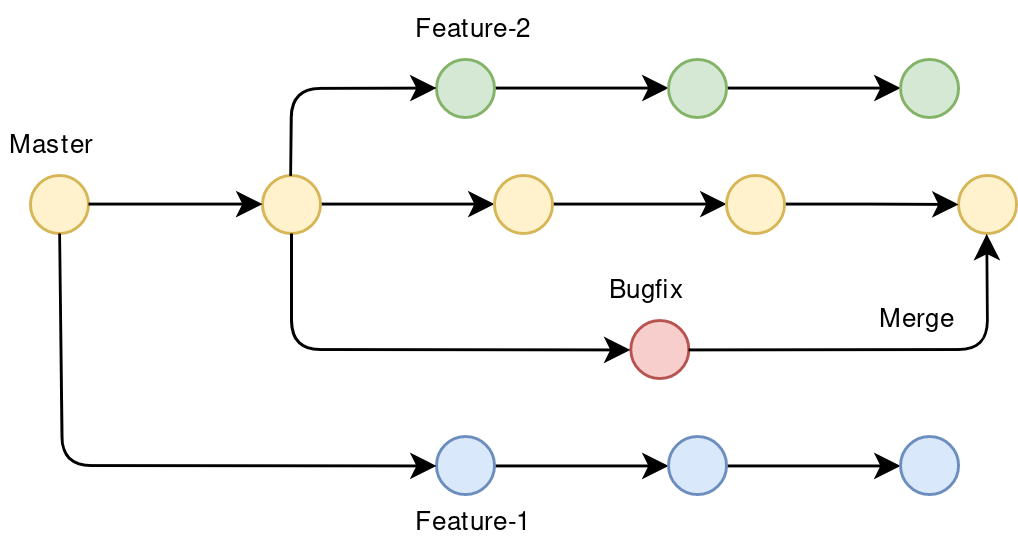
\includegraphics[scale=0.35]{./graphs/git-history-branch}
    \centering
    \caption{A Git commit history tree.}\label{fig:git-commit-tree}
\end{figure}

As shown in figure~\ref{fig:git-commit-tree} two developer can for example create their own branch on which they can work unimpeded.
If they finished their tasks and want to add their work to the master branch, they can now merge their changes.
Git then tries to automatically resolve any conflicts which might have emerged from editing the same lines in a file.
If that is not possible, it marks the conflicts and allows the user to manually correct them.
After this resolution a new \emph{merge commit} is created. A merge commit represents the merge of changes from two different branches.

With this methodology it is possible to work with many people or teams on the same project, without accidentally overwriting changes of another developer, whilst maintaining a clear history of all changes in the project.

Another important feature of Git is the possibility to set up a \emph{remote}.
A remote often acts as a centralized repository developers can \emph{push} their changes to or \emph{pull} changes from other developers.
This principle is called a \ac{cvcs} and is supported by many \acp{vcs}~\ref{version-control}.
System (CVS) 1 [52]
It can for example be a distinct server, which is attached to some kind of network that is accessible by the developers.
This feature allows developers to contribute to a project, as long as they have access to the remote's network.
Git also supports several protocols such as \ac{http} or \ac{ssh} to connect to a remote and thereby provide a simple user management layer.


\subsection{Git User Roles}
There exist two roles in Git, namely the \emph{committer} and the \emph{author}.
Every commit in Git contains the email addresses and the names of those two people.
The author of a commit is the person which actually contributed the changes in the files.
The committer is the person, which created the Git commit.
This is important to keep track of the original author of the changes.

Lets look at the case of an author contributing code to a project in an email with an attached patch file.
If a maintainer of the project now applies the patch file and commits without setting the author, the information about the original author would be lost.
Collected data indicates that in about 89\% the author and the committer are the same person.


\subsection{Internal Representation}
Git's underlying storage and management solution for files is commonly described as an mini \ac{fs}~\cite[p.~9]{book:pro-git}
In the following I will thereby refer to its file management layer as \emph{git-fs} and explain the most important aspects of it.

The representation of a single file in Git is called a \emph{blob} object~\cite[p.~56]{book:pro-git}.
A blob object is a file, which has been added to a \emph{git-fs}.
It is compressed and saved in the \inlinecode{.git/objects} directory under the respective \ac{sha1} hash of the uncompressed file.
As a result, there exists a blob object for every version of every file of the project.

The \ac{sha1} hashing for unique file identifier might seem unsafe at first, but the probability of a \ac{sha1} collision is really low, roughly $10^{-45}$.
In 2017 Google managed to force a collision in an controlled environment, but it is really unlikely to encounter such a collision under normal circumstances~\cite{techreport:sha-collision}.
This characteristic of \ac{sha1} hashing will become quite important in the design of the database later on.

As mentioned in the introduction~\ref{git-introduction} Git is used to store the state of a specific directory of an actual \ac{fs} running under an \ac{os}.
To represent a \ac{fs} or to simply bundle multiple Git blob objects together, Git uses the tree object.

A tree object is a file, which has a \ac{sha1} hash reference to all underlying blob and tree objects as well as their names and \ac{fs} permissions.
To represent a subdirectory, a tree simply holds a reference to another tree object.
With these tools Git manages to build its own basic representation of a \ac{fs}.

\begin{minted}[linenos]{text}
    100644 blob 11d1ee77f9a23ffcb4afa860dd4b59187a9104e9  .gitignore
    040000 tree ac0f5960d9c5f662f18697029eca67fcea09a58c  expose
    100644 blob 61b5b2808cc2c8ab21bb9caa7d469e08f875277a  install.sh
    040000 tree 8aaf336db307bdcab2f082bd710b31ddb5f9ebd4  thesis
\end{minted}
\begingroup
\captionof{listing}{A tree file example\label{lst:raw-commit}.}
\endgroup

As stated before the commit is utilized to provide an exact representation of a state of the repository's files and directories.
Just as blob object, the tree and commit files are also stored in the \inlinecode{.git/objects} directory under their respective hash.

\begin{minted}[linenos]{text}
    tree      cd7d001b696db430b898b75c633686067e6f0b76
    parent    c19b969705e5eae0ccca2cde1d8a98be1a1eab4d
    author    Arne Beer <arne@twobeer.de> 1513434723 +0100
    committer Arne Beer <arne@twobeer.de> 1513434723 +0100

    Chapter 2, acronyms
\end{minted}
\begingroup
\captionof{listing}{A commit file example\label{lst:raw-commit}.}
\endgroup

As you can see in listing~\ref{lst:raw-commit}, the commit is just another kind of file utilized by Git, which contains some metadata about a repository version:

\begin{itemize}
    \item The reference to a tree object, which represents the root directory of the commit's version of the project.
    \item A reference to one or multiple parent commits, to maintain a version history.
    \item The name and email address of the author.
    \item The name and email address of the committer.
    \item The timestamps with \ac{utc} offset for the commit and author date.
    \item The commit message. A message with arbitrary text from the committer.
\end{itemize}

The commit is the most important object for this thesis.
It contains crucial information such as the date of the commit as well as the email, which is needed to identify a contributor across several commits.

\subsection{Relevant Features}
Git provides a collection of high level abstraction tools to work with its underlying \ac{fs}.
In the following the most important features for data aggregation will be listed and briefly explained.

\begin{description}
    \item[HEAD] \hfill \\
        To mark the current checkout of an repository, Git utilizes a special marker called \emph{HEAD}.
        For instance, it is possible, due to this feature, to jump to the previous commit in history with \inlinecode{git checkout HEAD~1}.

    \item[diff] \hfill \\
        The diff is a tool to compare the state of two different commits in a repository.
        It allows to list all files which changed between those commits as well as showing the exact changes in the files

    \item[force push] \hfill \\
        Git allows to push to a remote with the \inlinecode{--force} flag, which is called a \emph{force push}.
        This enables the users to rewrite every commit in the whole history tree. If another user has a Git repository version
\end{description}


Git provides many more features, which are not necessarily important for data analysis, but which might need be taken into account when aggregating the data.
In the following some functionalities will be shown, which can lead to problems or irregularities in the gathered data.

\begin{description}
    \item[rebase] \hfill \\
        It is possible to \emph{rebase} branches. For instance a rebase can rewrite the commit history and change the branch point of a branch to another commit.
        This is for example a very powerful but also dangerous tool, as it implicitly changes the timestamps of the commits of the rebased branch.

    \item[filter-branch] \hfill \\
        In case somebody pushes a huge file, which significantly increases the size of the repository, or adds a file with secret information, for example a password file, Git provides the \emph{filter-branch} command.
        The filter-branch command removes a specified file from every commit in the history and thereby rewrites the history to the point, where this file was added to the repository.
        This command leads to similar problems as the rebase command, since it can severely change the history of a repository.

    \item[force push] \hfill \\
        Git allows to push to a remote with the \inlinecode{--force} flag, which is called a \emph{force push}.
        This enables the users to rewrite every commit in the whole history tree.
        If another user has the old Git repository version before the force push, they would now be incapable of simply pulling the newest version.
        Instead they would need to manually checkout the newest commit of the rewritten remote branch.

\end{description}


\section{Github}\label{github}
The biggest initial task for this thesis was the acquisition of data.
Selecting a data source was a crucial step as good data for analysis and evaluation is the backbone of this thesis. This chapter will list the requirements in detail and evaluate Github as a solution for these.

\subsection{Requirements}
The data source had to satisfy as many requirements as specified in Chapter~\ref{attack-models} as possible.

To accomplish a meaningful analysis of commit behaviour one needs a sufficient amount of commits.
For example one would need a few commits per weekday over a timespan of a month for a simple sleep rhythm analysis.
If there are only 20 commits for a user over the past month there is not enough data for a representative analysis.
To gain the most amount of commits one needs to get as many repositories a user contributed to as possible.

For analysis of companioned persons as described in Section~\ref{industrial-spy} it is crucial to find different user, which are likely to know each other.

To attack a company, as described in Section~\ref{industrial-spy}, or to spy on company members, as described in Section~\ref{employer-monitoring}, one needs as many repositories owned by the company as possible.
Thereby some kind of representation for a company should be available.
Ideally there should also be a list of all company members for evaluation purposes of data mining findings.

\begin{itemlist}{A recap of the requirements to the data source:}
    \item Realistic noise
    \item Real world data
    \item Large amount of repositories
    \item Access to all commits of each repository
    \item Access complete metadata for each commit
    \item Email to user association
    \item Methods to discover repositories a user contributed to
    \item Methods to discover companioned contributer
    \item A representation of a company
    \item Member of a company
    \end{itemlist}


\subsection{The Chosen One}
I decided to use Github as a data source, for it is not only convenient to find \acp{url} for cloning repositories, but also provides solutions most of the other requirements.
It hosts one of the biggest collection of open source projects with 64 million repositories, 24 million users and 1,5 million organizations~\cite{article:github-statistics}.
For comparison purposes: Gitlab, one of Githubs competitors, doesn't provide detailed usage statistics, but they state that they only host about 100000 organizations, which is remarkably less than Github~\cite{article:gitlab-help}.
Github also provides a well documented \ac{api} for querying its metadata.

One of the downsides of using Github is, that we don't have access to all metadata, as for example the full list of members for organizations or the internal team structure of organizations.
Another problem is old email addresses, which are not related to any account any longer, since all commits made with this email address are irrefutable.
Even though some ground truth is missing, I decided to use this approach as it is still the most promising way to gather as much data and real world noise as possible, compared to other open source hosting services.

\begin{figure}[H]
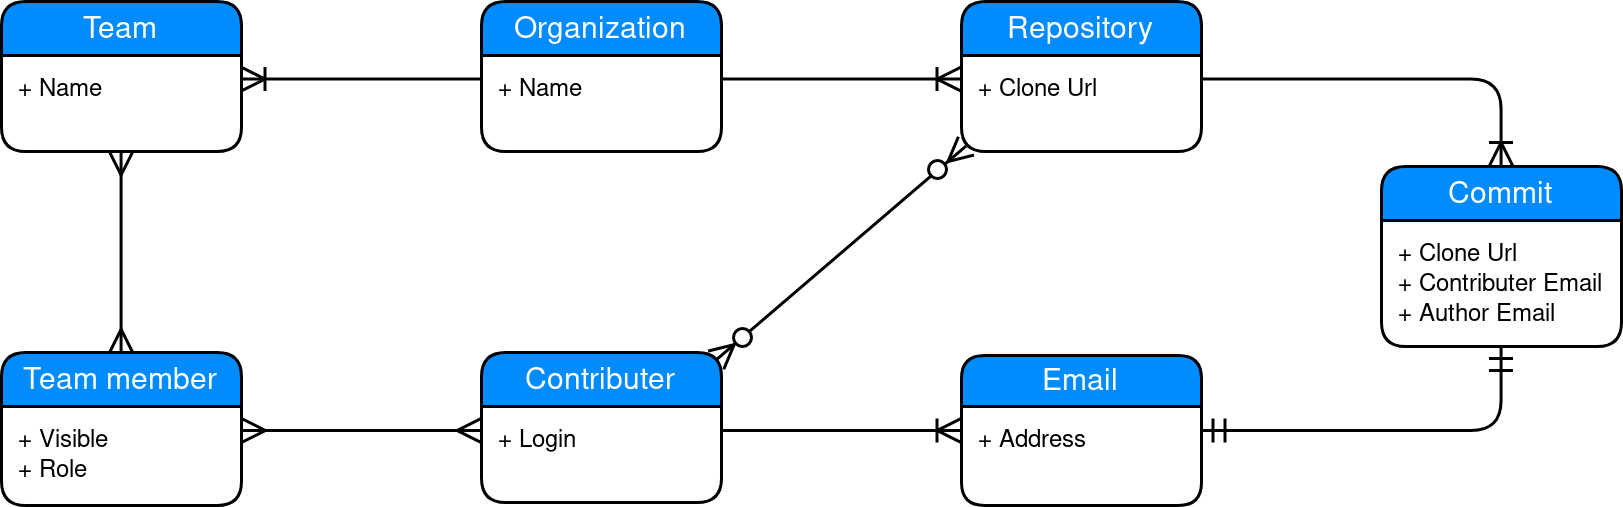
\includegraphics[scale=0.27]{./graphs/github-data-structure}
\centering
\caption{Simplified Github relationships.}\label{fig:github-relationship}
\end{figure}

\subsubsection{Github's features}
Github offers some features, which are convenient to for example find repositories a specific user contributed to or to find contributers which likely personally know each other.

\subsubsection{Stars}
The first feature is \emph{starring}. Every user can \emph{star} a repository to show that he likes a project.
The Github \emph{api} doesn't provide a method to get all repositories a user ever contributed to, it only allows to query the repositories actually owned or forked by a user, but it provides an endpoint to query all \emph{starred} repositories of an user.
In case a user stars a repository he contributed to, whilst not owning it, it is possible to get this repository with this feature.
Of course it is still no reliable way to get all repositories a user contributed to, but it is a solution approach to get at least a few of them.

\subsection{Follower}
Another feature is \emph{following}. Every user can \emph{follow} another user to get informed, if they do specific things like creating new repositories or \emph{starring} repositories.
By getting the followers or following, one might catch some friends of the user.
It is also possible that a user follows the owner of a repository he contributed to.
By using this feature it is thereby possible to catch some additional contributed repositories as well some friends of the user.

\subsection{Organizations}\label{github-organization}
The third feature are \emph{organizations}.
An organization is used to host projects under an account which is not necessarily led by a single natural person, but rather supports roles with different permissions and team structures.

This feature provides us with some important ground truth, but sadly a lot of information is not visible, as users have to actively opt-in, if they want to be publicly displayed as a member of an organization.
Additionally team structures can only be examined, if one is a member of the organization.
Despite not knowing all members of an organization, we still get some useful information to estimate the tendency of precision of our knowledge extraction algorithms.


\section{Data Aggregation}\label{aggregator}
As mentioned in Section~\ref{github}, I decided to use Github as my primary data source and to utilize their \emph{Github APIv3} for this purpose.
The aggregator and analysis program written for this thesis is named \emph{Gitalizer}.
In this section I will explain the technologies and methods used in the data aggregation process, the database structure and the interaction with Github's \ac{api}.
In the end some problems which occurred during the data collection will be shown as well.


\subsection{Existing solutions}

There are a number of existing solutions for accessing git metadata.
\todo{Add some references to existing solutions.}


\subsection{Database}\label{gitalizer-database}
To store the gathered Information I chose a \ac{sql} based solution.
PostgreSQL provides excellent tools to ensure a high consistency in your database, namely check constraints, as well as great support for working with times, time zones and locations.
The \ac{sql} database is used in combination with the \ac{orm} library \emph{SQLAlchemy}.

The basic schema created for the purpose of this thesis consists of five \ac{orm} models.
A model for commits, emails, repositories, contributors and organizations has been created.
The latter is only important to validate results and is not actually used for knowledge discovery, as this is Github specific data.

\begin{figure}[H]
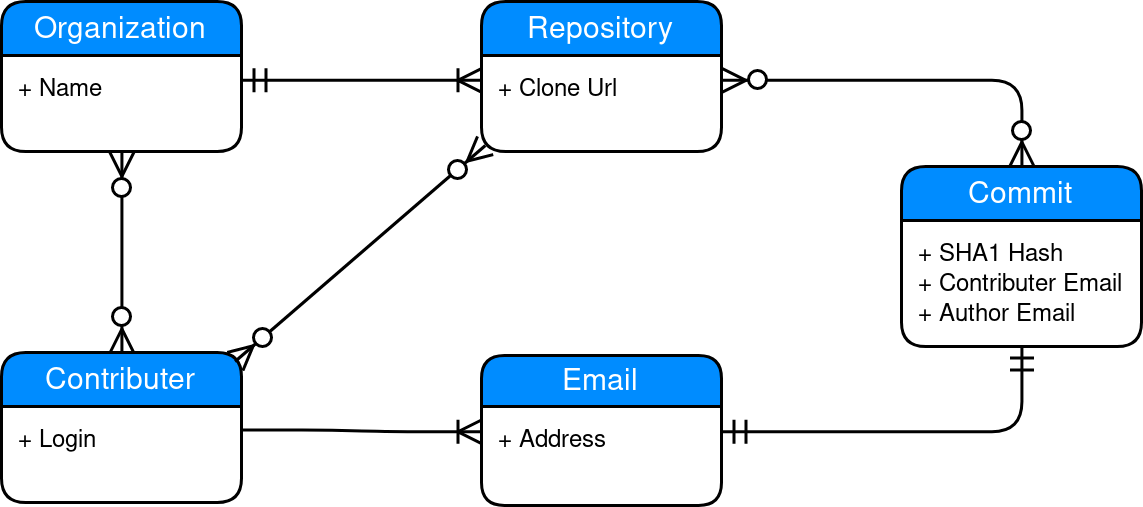
\includegraphics[scale=0.3]{./graphs/gitalizer-data-structure}
\centering
\caption{Gitalizer database relationships.}\label{fig:gitalizer-relationship}
\end{figure}

Every commit of each repository is saved in the database along with its \ac{sha1} hash and the two email addresses as in Listing~\ref{lst:raw-commit}.
It is important to note that there is a many-to-many relationship in figure~\ref{fig:gitalizer-relationship} between commits and repositories.
This feature prevents duplication of the same commits from forked repositories.
It is, for instance, a common practice to create a fork of a repository to develop without intervening with the main git repository of the project.
As described in Section~\ref{git-internal-representation} the probability of a \ac{sha1} collision is highly improbable.
By exploiting this feature, it is possible to enforce a unique constraint on the commit hash column, assuming that any duplicated commit hash actually results from a forked or copied repository.
The formula for calculating the probability of such a collision is:

\begin{equation}\label{eq:collision-probability}
    p \leq \frac{n(n-1)}{2} * \frac{1}{2^{b}}
\end{equation}

Without this mechanism it could be possible that the same commit of a contributor could be used multiple times as a result of repository forking.
After collecting 43 million commits from Github and actively ignoring obvious project forks, there are still 49 million references between commits and repositories.
This means that about 13\% of gathered commits result from forked repositories which can not easily be identified as such.
Considering Formula~\ref{eq:collision-probability}, the probability of a collision for 49 million hashes on the 160 bit \ac{sha1} hash would be about $8.21 * 10^{-34}$.

As stated above each commit is also saved with its respective email addresses.
There exists a one-to-many relationship between contributors and emails, as every contributor can obtain an unlimited amount of email addresses.
It is necessary to connect all email addresses commit to a specific contributor, to unambiguously assign all commit to their respective contributor.
This relationship does not have a \inlinecode{NOT NULL} constraint as it happens quite often that an email address can not be assigned to any person.
Looking at the collected data it appears that roughly 20\% of all collected email addresses from Github are no longer connected to an active user.

As stated in Section~\ref{github-features} Github provides a way to organize several people in organizations and teams.
As one of the goals of this thesis is to see if it is possible to detect member of an organization in open-source projects, a model for organization has been created as well.
This data can then be used to check against the results of this research's results.


\subsection{Gitalizer}
The Program written for this thesis features data aggregation, preprocessing, knowledge extraction and visualization.
Gitalizer uses a PostgreSQL database for data storage and data consistency checks as described in~\ref{gitalizer-database}.
For interaction with the Github \ac{api} the \emph{PyGithub} library is used, which provides a convenient abstraction layer for requests and automatically maps \ac{json} responses to \emph{Python} objects.

The data aggregation module of Gitalizer is capable of several approaches for gathering data.
In the following we will look at those approaches in detail.

\begin{description}
    \item[Git repository]\label{stand-alone-repository-scan} \hfill \\
        Gitalizer can scan any git repository from a \ac{ssh} or \ac{http} \acs{url} as long as the current user has access to it.
        The repository is cloned into a local directory. After the cloning finished the actual scanning process begins.
        During the scan, we git checkout the HEAD of the current default branch for this repository and walk down every reachable commit of the Git history.
        The program saves all available metadata for each commit in its database, namely the emails, timestamps as well as additions and deletions to the project in lines of code.

        After this scan we are still missing a lot of information.
        There exists no unique identifier of an author or committer, as names may change or can be ambiguous and a single person can have multiple email addresses.
        The problem with the simplicity of Git is that there exists no concept of an user.
        Thereby we cannot easily link several email addresses to a specific contributor without additional metadata.


    \item[Github Repository]\label{github-repo-scan} \hfill \\
        To tackle the problem of missing metadata in~\ref{stand-alone-repository-scan}, I used the Github \ac{api} to get some of the missing metadata.
        The general approach is the same as in the previous scan method. The repository is cloned and locally scanned.
        However, a request to Github is issued every time an email is found, which we do not already have linked to a contributor.
        Github allows to link multiple email addresses with a single user account and automatically references the respective user in their own \ac{api} commit representation.
        With this additional metadata we gain ground truth about the identity of an author or committer.

        Anyway this approach does not work, if the user of a commit removes the email, which has been used for the commit, from his account or if the user completely deletes their account.
        If this happens and the email contributor relationship has not already been created, there is nothing that can be done and these commits need to be handled later on in the preprocessing of the data.

    \item[Github User]\label{github-repo-scan} \hfill \\
        To try getting all repositories of a specific user, a new functionality has been added, which highly utilizes the Github \ac{api}.
        At first several requests are issued to get all repositories of the specified user, as well as all starred repositories of this user.
        During the repository exploration, every relevant repository is added to a shared queue, lets call it ``repo-queue'', which is then processed by a multiprocessing pool of workers.
        Each worker process pops another entry from the ``repo-queue'' and scans a single repository as described in~\ref{github-repo-scan}.


    \item[Connected users and organizations]\label{github-repo-scan} \hfill \\
        For detection and analysis of connections between contributors over multiple repositories additional user repository discovery as described in~\ref{requirements}, another feature has been added to Gitalizer.
        Gitalizer is able to achieve this by not just scanning a single user, but also scanning the repositories of all following and followed users as described in~\ref{github-user-scan}.
        For this task two different worker pools are utilized.
        The user discovery pool is initialized with a shared queue, lets call it ``user-queue'', of all users we need to look at.
        This worker pool simply searches for relevant repositories of each user and passes the repository \ac{url} to a second shared queue.
        The second pool then processes this ``repo-queue'' as described in~\ref{github-repo-scan}.

        For organizations it's nearly the same approach.
        Initially all repositories, which are owned by the organization, are added to the ``repo-queue''.
        All publicly visible organization members are then added to the ``user-queue'' and processed as described above.
\end{description}


\subsection{Database optimization}
As the database kept growing, it became the bottleneck in the aggregation process several times.
As a result, adjustments in the database schema, PostgreSQL parameter tweaking and migration to better hardware were necessary.
The first considerable slowdown occurred after reaching about 12~\acp{gb} of data.
At this stage the database write and read operations took longer than the actual aggregation process and the whole machine started to become unresponsive because of high I/O load.

The performance of the database then needed to be continuously tweaked in several steps.
The first countermeasure was the reduction of commits using deduplication by using the features of the \ac{sha1} hash as stated in Section~\ref{database-design}
The ignoring of forked repositories reduced the amount of entries in the relation table between commits and repositories by another 26\%.

The next performance boosts were achieved by disabling or loosening several fail-safe mechanisms of PostgreSQL, namely `synchronous commit' and `write ahead' parameter, which are designed to save data on a system crash.
As there is no important or critical data handled it was acceptable to pass on these mechanisms, and trade safety for performance.

\begin{figure}[H]
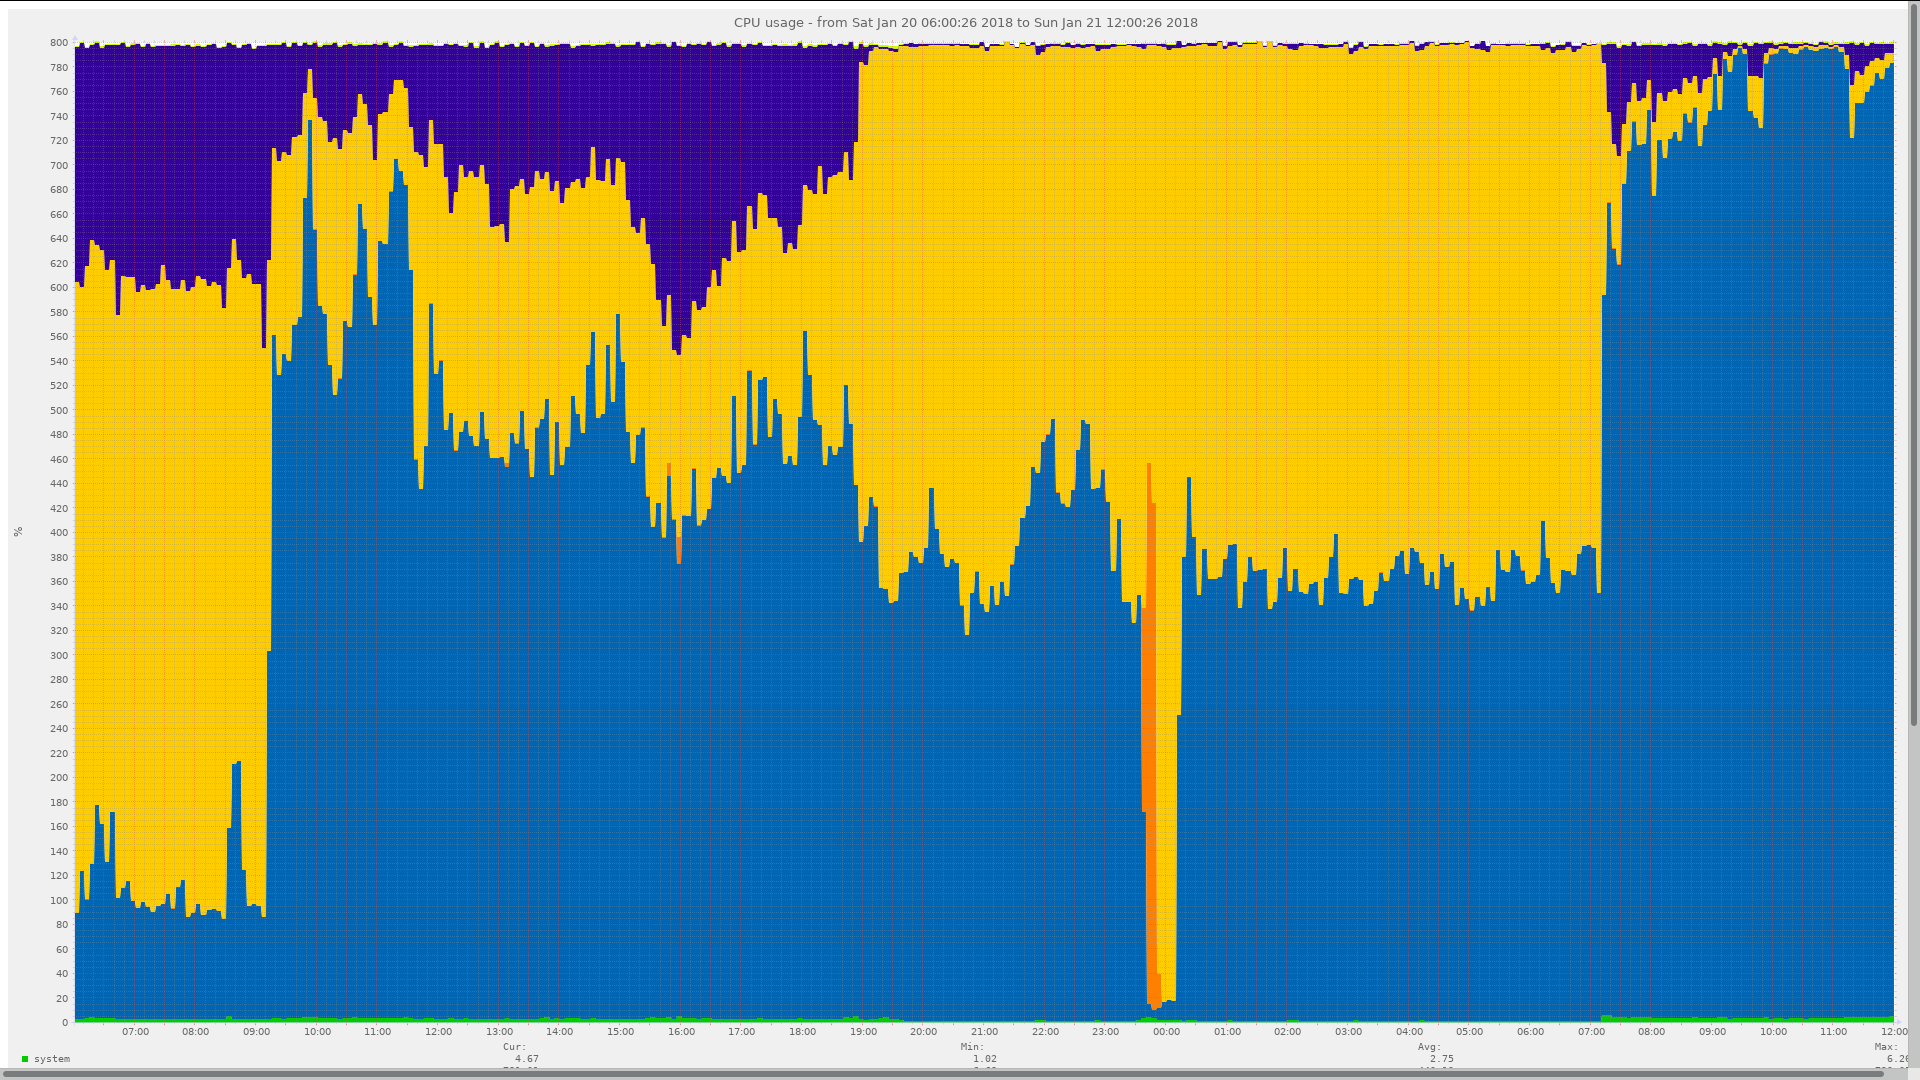
\includegraphics[scale=0.22]{./graphs/server-graphs/query-refactoring}
\centering
\caption{The CPU load of the aggregation server during optimization.}\label{fig:cpu-load}
\end{figure}

After renting a root server and deploying Gitalizer onto it, the aggregation process worked really well, until the database size hit about 25~\ac{gb}.
In Figure~\label{fig:cpu-load} you see the overall \ac{cpu} load right before optimizing several \ac{sql} queries by caching intermediate results and increasing the cache size of PostgreSQL.
The dark blue represents the I/O wait time while the light blue represents the actually used processor capacity by the aggregator.
Due to complex and numerous \ac{sql} queries the server became partly unresponsive and the aggregation process began to stall.

After many improvements the server can now run with 16 worker threads and roughly 38~\ac{gb} of data without any signs of slowdown whilst using the rate limit to capacity.


\subsection{Incremental aggregation}
To ensure a constantly up to date database, Gitalizer needed to be capable of fast rescans of repositories.
The initial scan of a repository always includes cloning, scanning the whole repository and writing it into the database.
After a repository is scanned completely at least once it is marked as as such and will never by completely scanned again.
All following runs then only clone the repository and scan the newest unknown commits.
These are discovered by performing a breadth first search until no new nodes are found.

\begin{figure}[H]
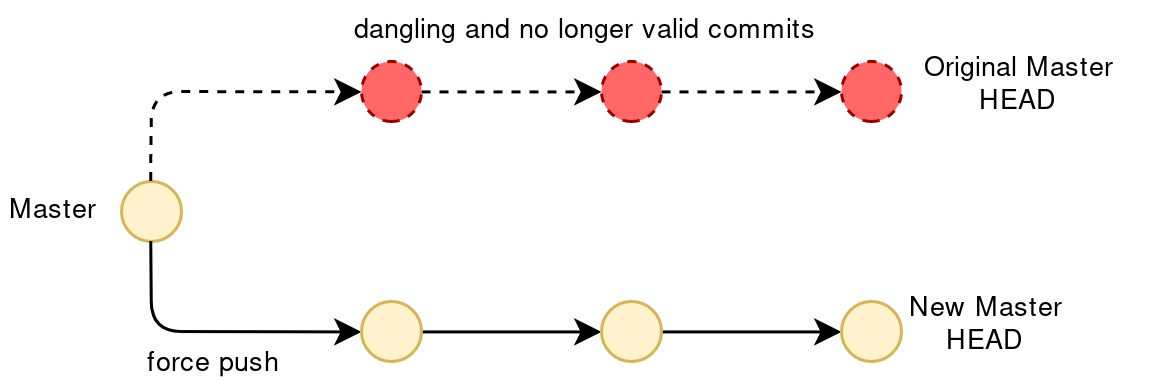
\includegraphics[scale=0.3]{./graphs/git-history-rewrite}
\centering
\caption{Gitalizer database relationships.}\label{fig:gitalizer-relationship}
\end{figure}

As explained in Section~\ref{more-git-features} it is possible to rewrite commits and force push them.
This scenario needs to be explicitly handled since force pushes can completely alter the history of a git repository, which can subsequently lead to a split in the Git history and leaves dangling commits.
As the complete history of a repository is stored inside the database, Gitalizer needs to detect a force push by walking down the git history tree until it finds known commits.
If any of these commits has children, which are not in the newly scanned commits, a force push took place and the old commit history has to be truncated, since it is now outdated and irrelevant.
An example scenario can be seen in Figure~\ref{fig:gitalizer-relationship}, where all red commits represent the old commit history, which needs to be truncated.


\subsection{Problems}
During the development of the data aggregator I experienced a few problems and edge cases which needed to be handled.
The earliest and most delaying problem was the rate limit of the Github \ac{api}, which limits to 5000 requests per hour.
Beside this rate limiting there also is an abuse detection mechanism, which triggers, if too many requests are fired in a short amount of time.
The solution for this problem resulted in various hacks, which include random wait times to detain those mechanisms from triggering.

The first version of the aggregator didn't clone and scan the repository locally, but rather gathered all information from the Github \ac{api} endpoints.
This approach worked well until the aggregator hit the official repository of \emph{Nmap}, which has about 11.000 commits and took over three hours to scan.
Soon I realized that this would severely slow down my research and I then started to continuously minimize the amount \ac{api} calls issued by Gitalizer.
A connected user scan of my own Github account led to about 600.000 commits and took about one and a half day on the final working version of Gitalizer, to provide you with a reference of scale.

After implementing multiprocessing, I managed to hit the rate limit again, as I was now issuing requests to the \ac{api} with multiple threads.
To fix this issue I implemented a wait and retry wrapper around every single function call or object access, which triggered a call to the Github \ac{api}.
Afterwards the aggregator was capable of running multiple days without worker processes silently dying or finishing with incomplete data.

Fine tuning the edge cases and the handling of the \ac{api} took about 3 months, since there were many problems such as unpredictable error responses from Github, missing data in queries or simply unknown or broken encodings in Github's metadata.

A big throwback became apparent as I discovered that PostgreSQL automatically normalizes \ac{utc} timestamps with any offset to the \inlinecode{UTC +0} timezone.
As a result of this normalization, the exact time of the commit admittedly stays the same, but the crucial metadata about the offset is lost.
As a consequence the commit model needed to be adjusted, as the \ac{utc} offset had to be stored explicitly, and the whole commit aggregation process was started from scratch.

Another problem occurred during the local scanning of the repositories.
The library used for interaction with Git \emph{libgit2} issued \emph{stat} Linux syscalls during a diff operation for each file, which changed between those commits, to check if there were any local uncommitted changes.
Anyhow the repositories, which were locally scanned, were cloned with \emph{bare} mode.
This means that there exists no project root directory, but rather only the git internal representations of those files, which makes the behaviour stated above unnecessary and unwanted.
As a result all processes slowed severely down due to high I/O wait times, because of stat syscalls on non existent files.
Luckily after reporting the issue~\footnote{`Unnecessary syscalls on bare repository' github.com, https://github.com/libgit2/libgit2/issues/4480 (accessed, 25.04.2018)} it was resolved in a week and I was able to continue developing with my own compiled version of the libgit2 library.



\chapter{Implementation}\label{implementation}
After collecting all necessary data as shown in Chapter~\ref{data}, I will now begin to analyse this data.
In this chapter the approach for several attacks, as listed in Section~\ref{attack-models} will be introduced and the attack's goals recapitulated.
The possible applications for the gained knowledge will be stated and the implementation of and requirements to the respective algorithm will be explained for each attack.

\section{Holiday and Sick Leave Detection}

The goal of this attack is to detect miss-out by looking for anomalies in the work day patterns of a developer.

Due to possible fluctuations or changes in work routine, one requirement to this algorithm is the flexible detection of regular work patterns.
It must have the ability to adjust to a changing work pattern, but at the same time it needs to be capable of detecting anomalies in this pattern.

The input for this analysis is the intersection between all commits from the considered repositories and all commits from the considered contributors.
The commits' metadata used for this analysis are timestamps as well as additions and deletions in lines of code.

\begin{figure}[H]
    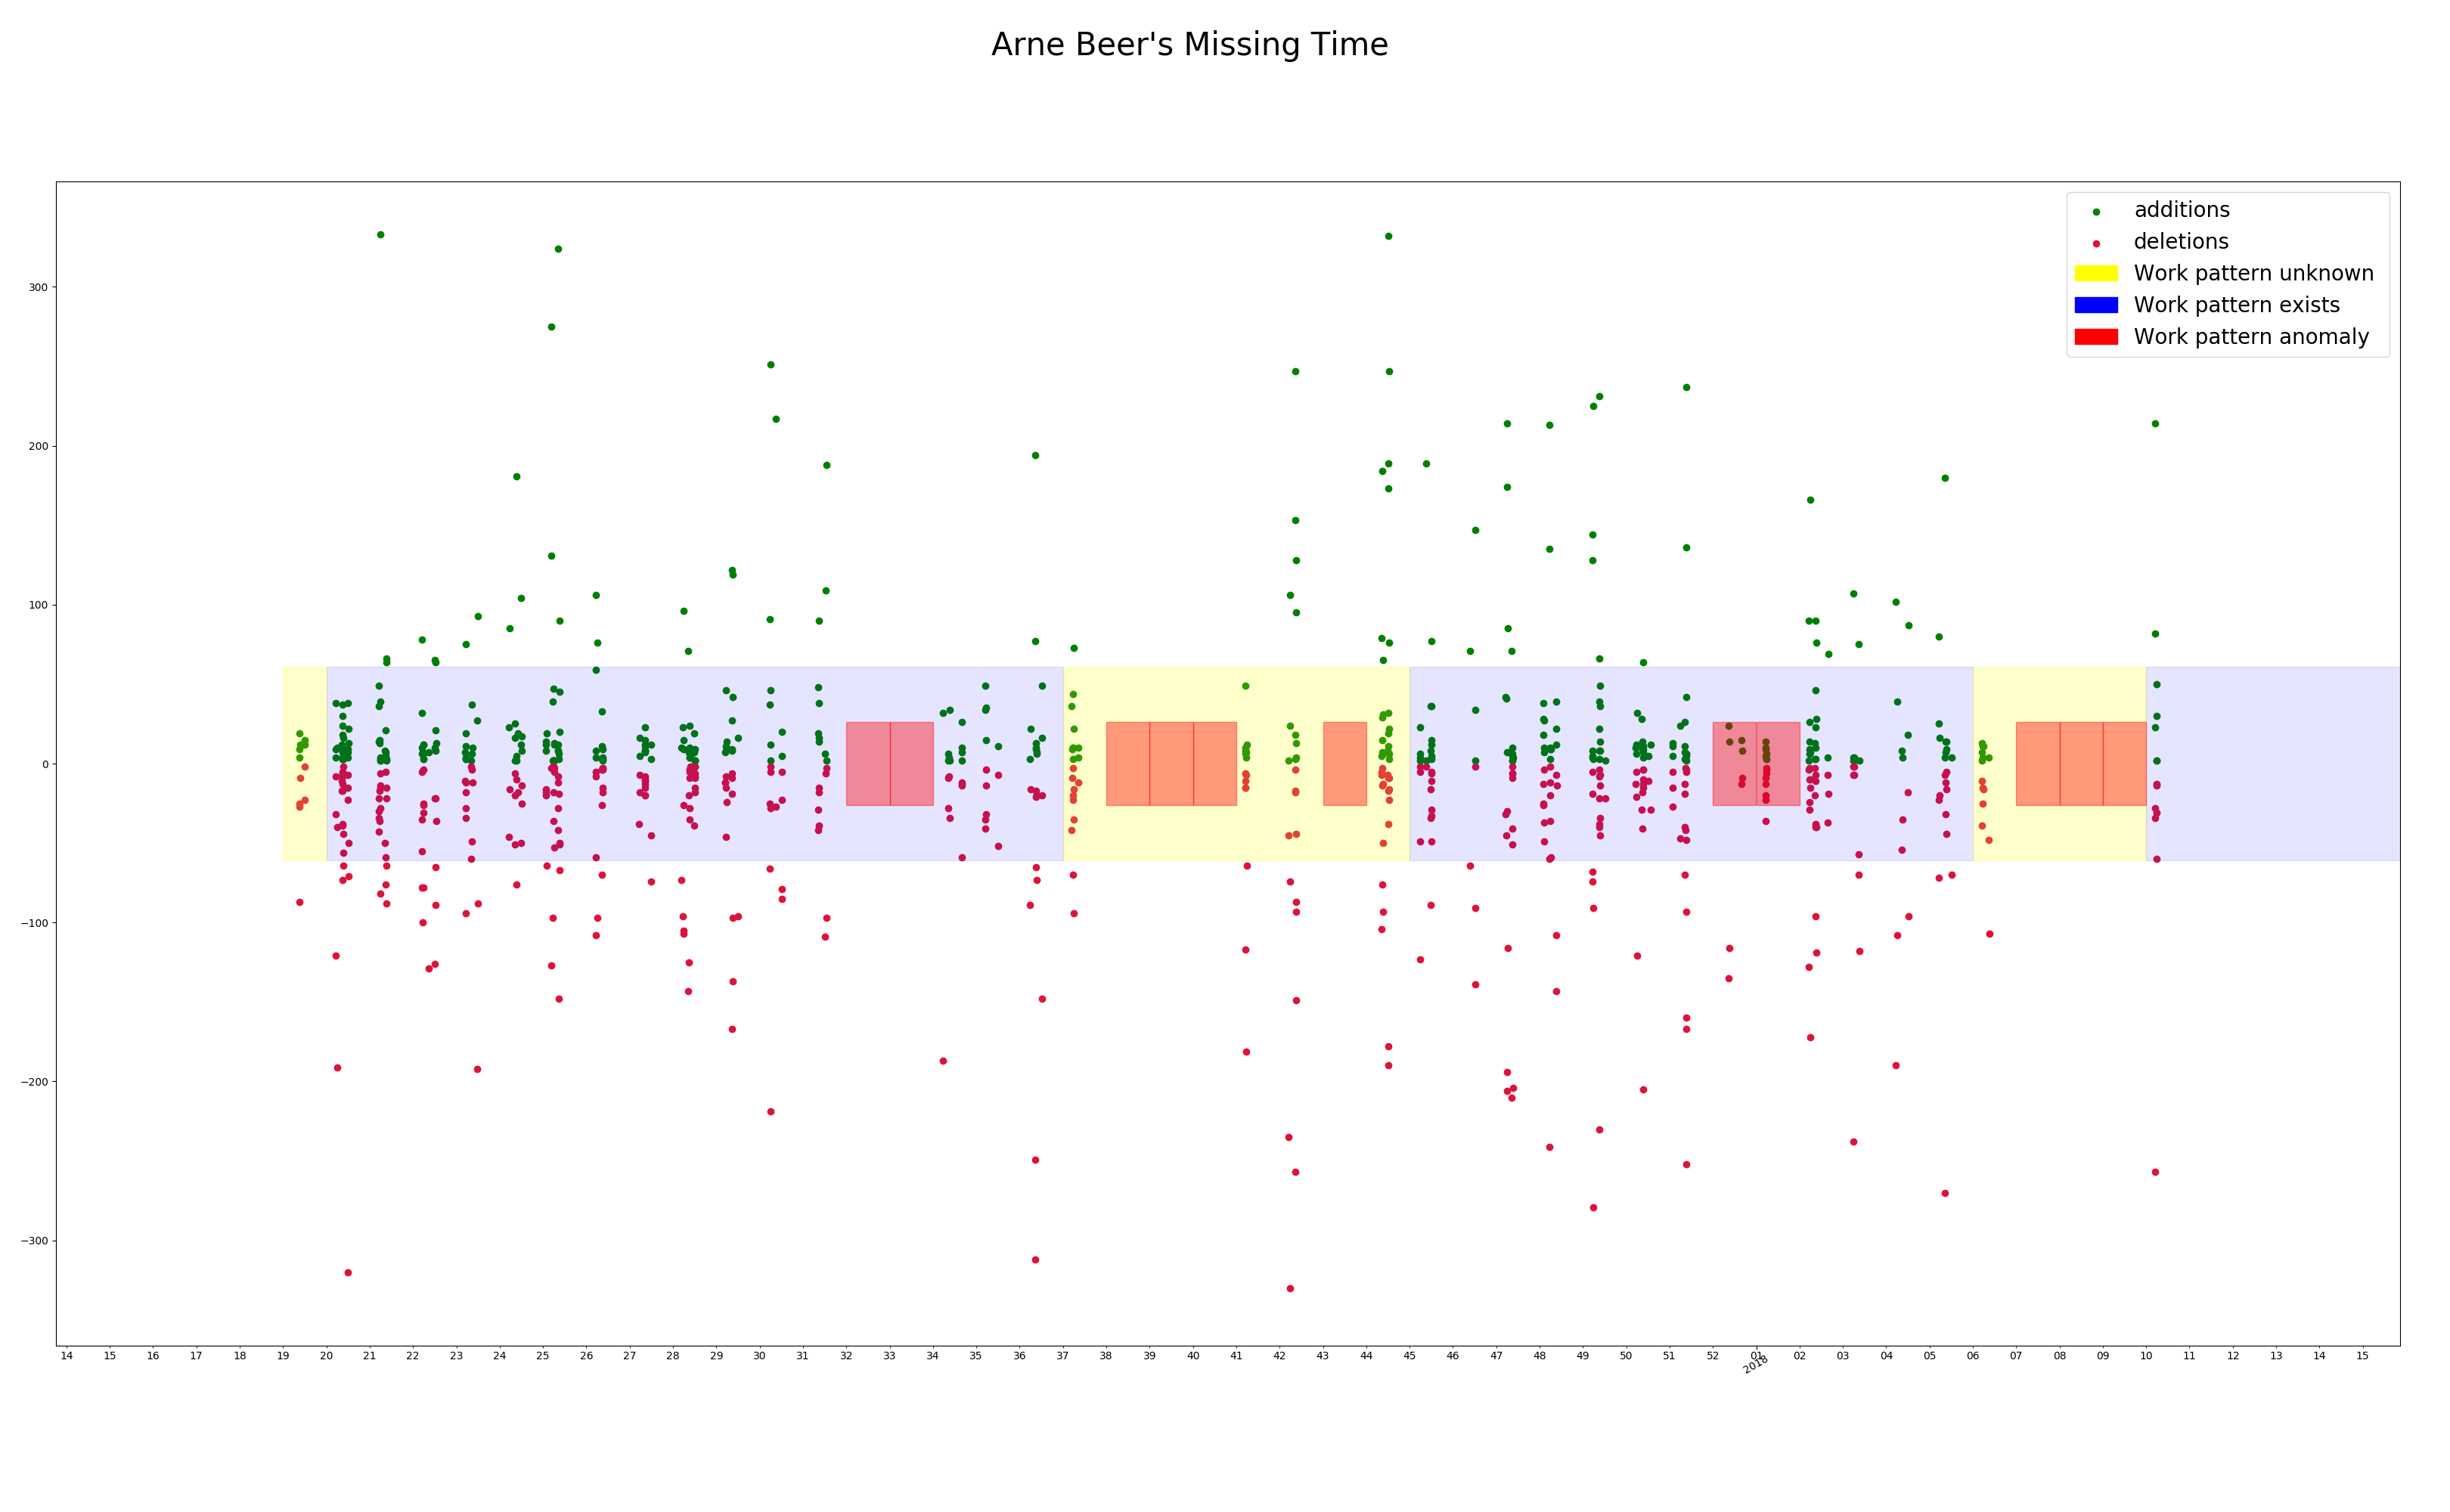
\includegraphics[scale=0.20]{./graphs/analysis/work-time-analysis}
    \centering
    \caption{The work time analysis of an employee.}\label{fig:missing-time}
\end{figure}

It is really difficult to measure productivity in lines of code or in the number of commits made by a person, as they do not necessarily display the amount of work, which has been put into this code.
As a result I decided, that a day counts as a work day as long as at least a single commit is created during the day.
Before performing the actual analysis, the data is preprocessed into an easier to handle format.
For each week of the last year a vector representing the weekdays is created.
Afterwards each day, a commit has been made on, is marked as a working day.
The preprocessed data is thereby equivalent to which days a contributor worked on, ordered by the week of the year.

\begin{minted}[linenos]{python}
def analyse(weeks):
    prototype = None
    for index, week in weeks.items():
        next_six_weeks = weeks[index:index+future_lookup]
        if not prototype:
            # Check whether there is a prototype in the next few weeks.
            prototype = find_prototype(next_six_weeks)

            # Check if this specific week is a anomaly
            check_anomaly(prototype, week)

            continue

        prototype_exists = prototype_exists_in_next_weeks(next_six_weeks)
        if not prototype_exists:
            # We couldn't find the prototype in the next few rows
            # Try to find a new prototype
            prototype = find_prototype(next_six_weeks)

        check_anomaly(prototype, week)


def check_anomaly(prototype, week):
    if week.working_days == 0:
        save_anomaly(week)

    if prototype is not None:
        different_days = week.working_days - prototype.working_days
        // A single day variance is acceptable
        if different_days >= 1:
            save_anomaly(week)

\end{minted}
\begingroup
\captionof{listing}{Miss-out analysis algorithm.}\label{lst:miss-out-algorithm}
\endgroup

The analysis of the data is a chronological scan of all work weeks for a specific user.
The algorithm inspects every week work pattern of a given interval, which has been set to a year for this analysis.
At the beginning, the algorithm tries to find a new \emph{prototype}.
A prototype is a representative week work pattern, which resembles the average work day pattern of the next weeks.
This is performed in the function \inlinecode{find\_prototype} in Listing~\ref{lst:miss-out-algorithm}.


\begin{minted}[linenos]{python}
def find_prototype(self, weeks, threshold):
    """Look at the first few weeks to find a new prototype."""
    # Create an entry for each pattern and count the occurrences of this entry
    occurrence_counter = {}
    for _, week in weeks.iterrows():
        pattern = week.pattern
        if pattern not in occurrence_counter:
            occurrence_counter[pattern] = {
                'prototype': week,
                'count': 1,
            }
        else:
            occurrence_counter[pattern]['count'] += 1

    # Get the prototype for the pattern with the most occurrences
    #
    # If there is no week which solely has the most occurences, return None.
    # In this case we can't predict a proper prototype.
    max_count = 0
    invalid = False
    prototype = None
    for _, item in occurrence_counter.items():
        if item['count'] > threshold and item['count'] > max_count:
            prototype = item['prototype']
            max_count = item['count']
            invalid = False
        elif item['count'] == max_count:
            invalid = True

    if invalid:
        return None

    return prototype
\end{minted}
\begingroup
\captionof{listing}{Miss-out analysis algorithm.}\label{lst:prototype-detection}
\endgroup

This function, which can be seen in Listing~\ref{lst:prototype-detection}, performs a simple iteration over a fix amount of future weeks, to find a work day pattern occurring more often than a given threshold.
If a prototype is found, we are capable of identifying anomalies that deviate from this pattern.

For each following week it is then firstly checked if this week is a anomaly in regards to the current prototype.
Anomalies are simply detected by comparing the amount of working days of the prototype and the considered week.
The difference in the working patterns is not suitable for this analysis, as it produces too many false positives for employees with flexible work time.

Secondly it is checked if a week identical to the prototype exists in the near future.
If there is no such week, the current prototype is reset and a new prototype needs to be found again.

In case no prototype can be found, anomalies cannot be easily identified, as there exists no pattern to check against.
Only obvious anomalies, namely weeks without a single work day, will then be marked as such.


\section{Sleep Rhythm and Working hours}

The next attack aims to extract information about the working hour behaviour of a target.
This should be achieved by displaying the pattern of the target in form of a weighted scatter plot and by comparing those patterns between several targets.
Additionally the detection of anomalies such as automated programs, which contribute to a project on a regular basis, will be conducted.

A clustering will be performed to find anomalies, common patterns and to evaluate the results of this analysis.
As we are only interested in contributors with a representative amount of commits, all contributors with less than one hundred commits in the last year have been excluded.
This reduced the amount of considered contributors from 175.000 to about 10.300.


\subsection{Implementation}\label{punchcard-implementation}

The data used for this analysis are the commit timestamps of the target, as well as the Github employee information for verification.
These commit timestamps are then converted into a different format, which represents the occurrences of commit per hour per weekday over the last year.
The result is a simple vector with length 168, which corresponds seven days with 24 hours each.
I will refer to this representation hereafter as a \emph{punchcard}.

\begin{minted}[linenos]{python}
def preprocess(commits):
    punchcard = [0] * 168
    for commit in commits:
        hour = commit.commit_time.hour # returns 0-23
        weekday = = commit.commit_time.weekday() # returns 0-6

        index = weekday*24 + hour
        punchcard[index] += 1

\end{minted}
\begingroup
\captionof{listing}{Data preprocessing}\label{lst:puchcard-preprocessing}
\endgroup

The data transformation is simply achieved by incrementing the field of the respective weekday and hour by one for each commit, as can be seen in~\ref{lst:puchcard-preprocessing}.
The resulting punchcard vector is then stored in the database for faster and easier analysis in the next steps.

\begin{figure}[H]
    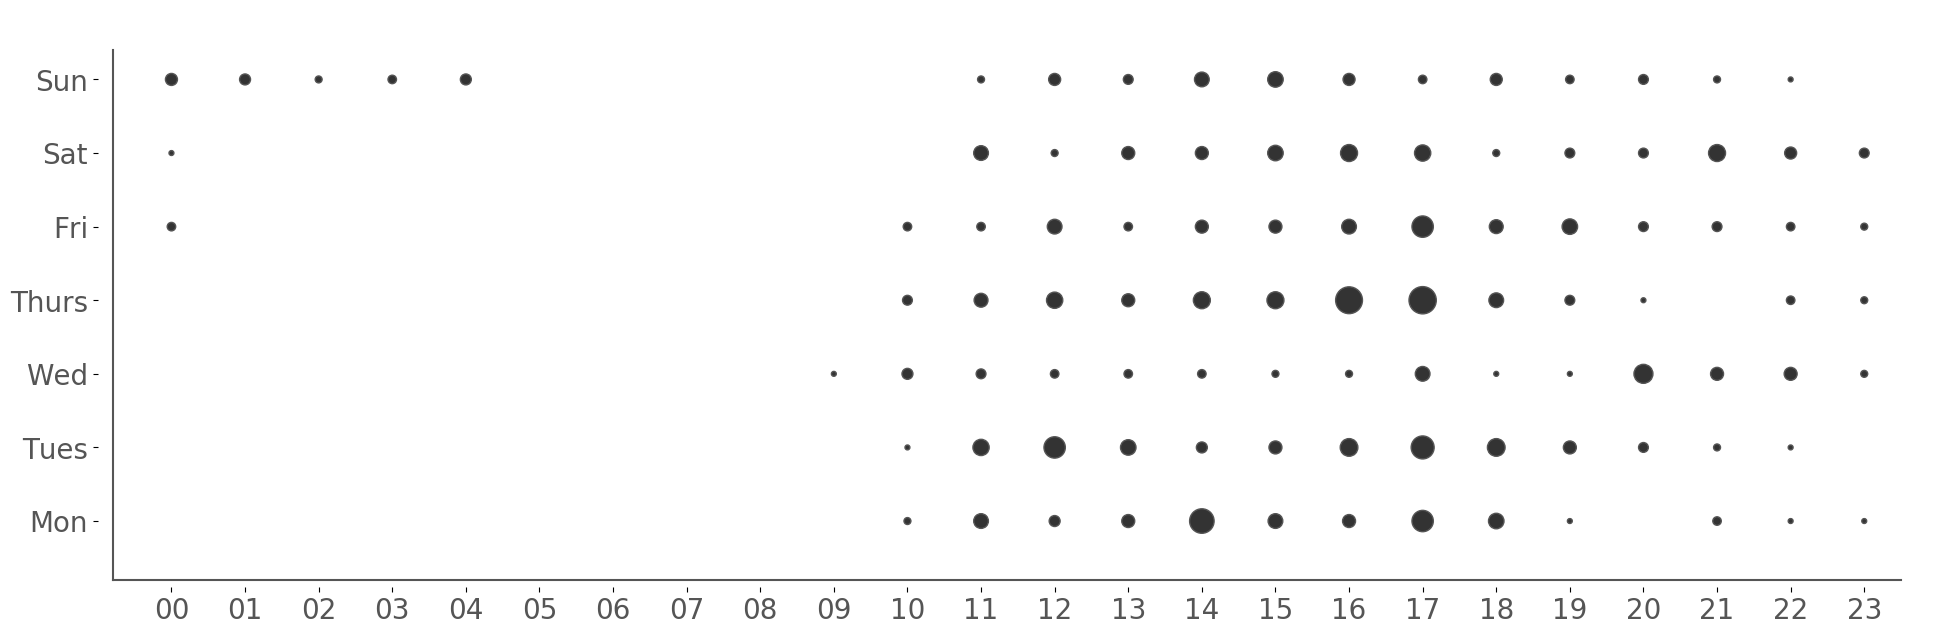
\includegraphics[scale=0.32]{./graphs/analysis/ordered-punchcard}
    \centering
    \caption{Punchcard of the author.}\label{fig:working-hour-rhythm-author}
\end{figure}


\subsection{Punchcard Clustering}

To find common work patterns, several cluster algorithms have been used on the aggregated data.
The Python \emph{scikit} framework has been used for this purpose, as it features nine different clustering methods and provides good documentation and abstraction from the underlying clustering logic~\footnote{`Clustering' scikit-learn.org, http://scikit-learn.org/stable/modules/clustering.html (accessed, 24.04.2018)}.

For the task of finding similar punchcard patterns in the data, a clustering algorithm is required, which can operate on a high-dimensional dataset with an unknown amount of clusters
Scikit provides three different clustering algorithms, which can handle an unknown amount of clusters.

\subsubsection{Mean Shift}\label{mean-shift}
Mean shift is a clustering methods, which performs an operation similar to a gradient descent, by which all adjacent data points are shifted towards their center~\cite{article:mean-shift}.
The goal of this algorithm is to find a representative centroid for each cluster and assign each data point to a cluster.
Unfortunately this methodology proves to be too aggressive for the current data.

\begin{figure}[H]
    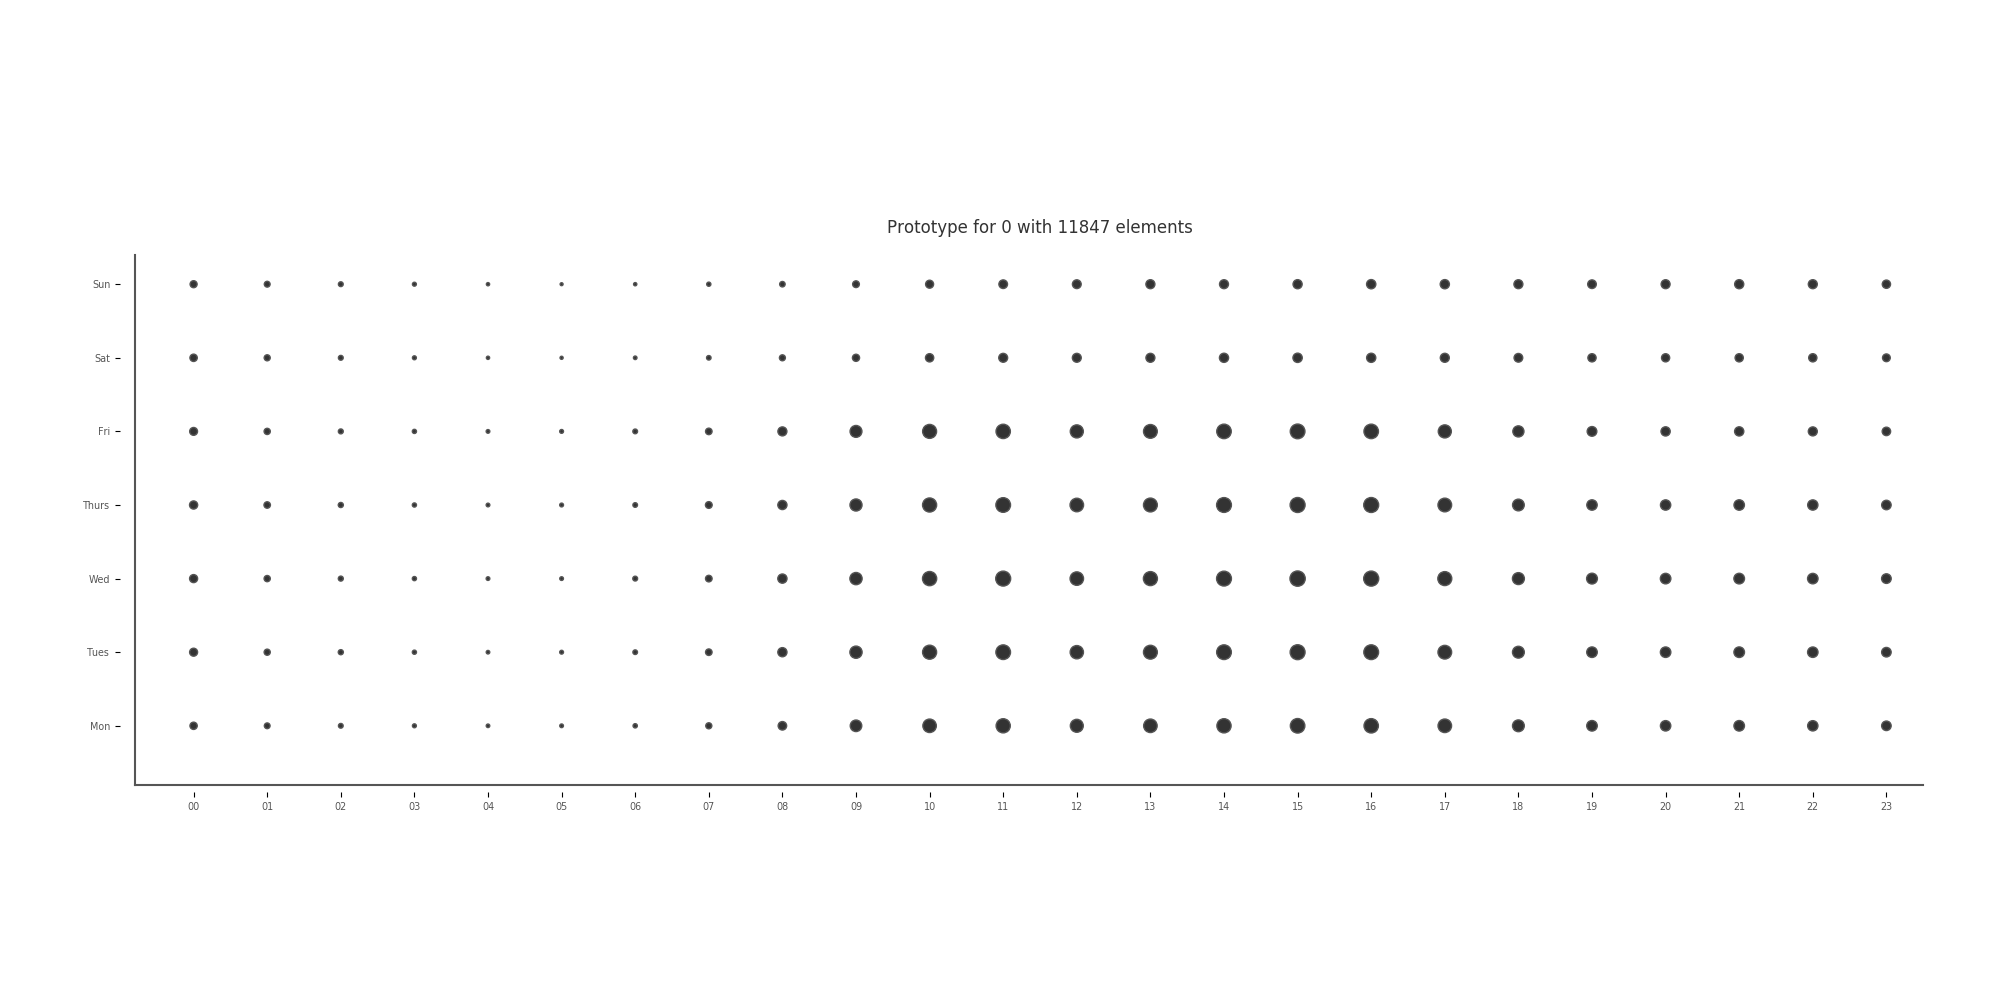
\includegraphics[scale=0.32]{./graphs/analysis-mean-shift/supercluster}
    \centering
    \caption{Super cluster centroid found by mean-shift clustering.}\label{fig:mean-shift-super-cluster}
\end{figure}

Despite trying a wide range of values for the bandwidth, which is the measure of distance used for detecting adjacent points, this algorithm always created a super cluster, which containes more than 89\% of all data points.
Such a super cluster can be seen in Figure~\ref{fig:mean-shift-super-cluster}.
The other 11\% were invariably small clusters representing extreme outlier or strange patterns, which do not resemble any of the expected patterns for normal work shift or leisure time developers.
An example for such an extreme outlier can be seen in Figure~\ref{fig:mean-shift-outlier}.

My assumption is, that the density of data points is too high and that they are too equally distributed around the centroid of the super cluster, for the major part of the provided data.
Thereby all those data points are slowly shifted to this single centroid.
As it is difficult to debug 168-dimensional space, I decided that a profound analysis would be too time consuming and to try the next solution.

\begin{figure}[H]
    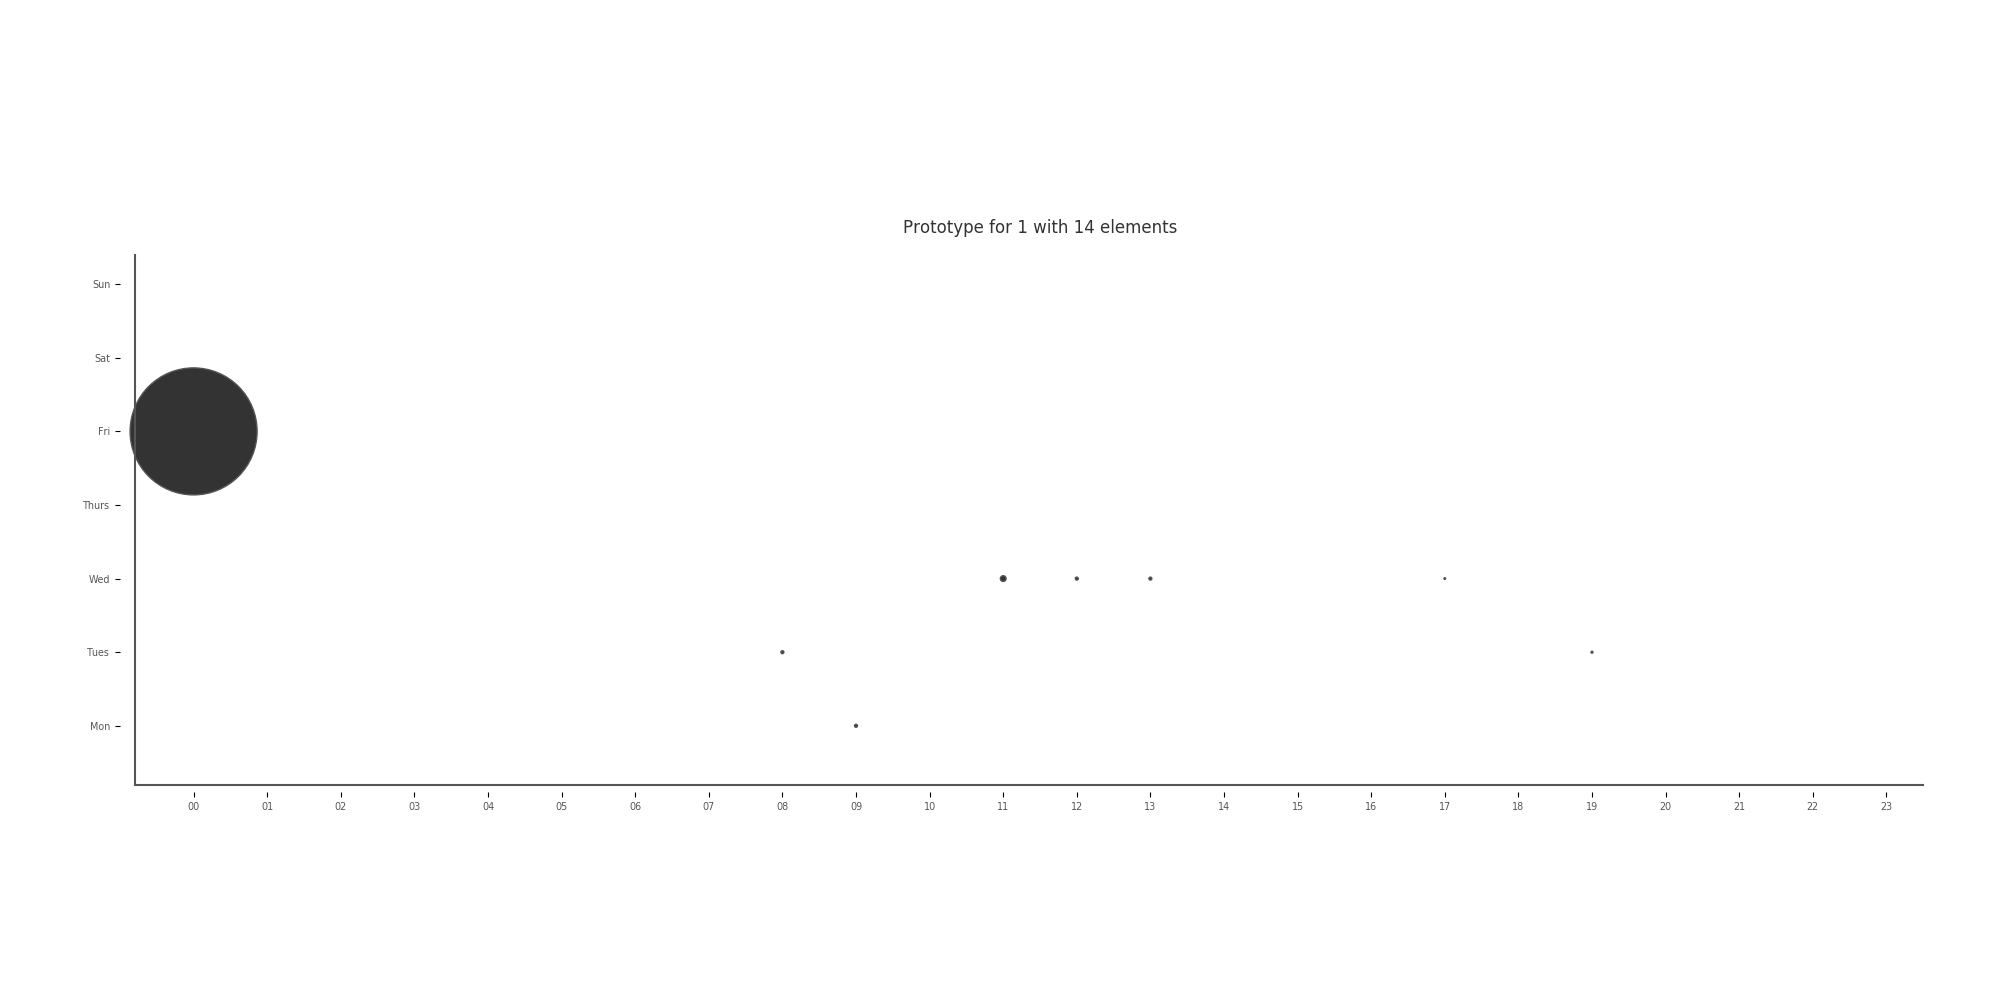
\includegraphics[scale=0.32]{./graphs/analysis-mean-shift/outlier}
    \centering
    \caption{Extreme outlier centroid found by mean-shift clustering.}\label{fig:mean-shift-outlier}
\end{figure}

\subsubsection{DBSCAN}
The \ac{dbscan} clustering algorithm operates by creating clusters of transitively connectable data points within a specific maximal acceptable distance between adjacent points.~\ref{inproceedings:dbscan}.
It is highly scalable and performant, even for large data sets, which made it my first choice.
Unfortunately it produces very similar results to the mean shift clustering algorithm~\ref{mean-shift}, since it finds a super cluster very similar to Figure~\ref{fig:mean-shift-super-cluster}.

I assume that this algorithm suffers from similar problems as the mean shift approach, which are high density and equal distribution of data points without clear borders.
Thereby the algorithm manages to reach the most part of all data points transitively from a single starting point.
When supplied with smaller values for the maximal acceptable distance between data points, it creates a huge amount of mini clusters, just as expected.

This algorithm also manages to find extreme outlier clusters, but it is not suitable for the purpose of this thesis, due to the extremely low granularity on the data inside the super cluster.


\subsubsection{Affinity Propagation}
The Affinity Propagation algorithm considers similarities between all data points to find clusters~\cite{article:affinity-propagation}.
This clustering algorithm features a promising approach, as it utilizes a method similar to message passing, to find an \emph{exemplar}, which resembles the representative of a cluster, and its surrounding cluster member.

Affinity Propagation was the only available clustering method that was detailed enough to find interesting patterns without creating a super cluster.
About 200 different patterns have been discovered using this methodology.
However it has to be noted, that this clustering method is sometimes a little too detailed, since it split very similar patterns into two or more different clusters.

Additionally, the memory requirements for this algorithm scale quadratically for non-sparse sets with the number of the data points~\cite[p.~ii]{article:affinity-propagation}.
About 12 \ac{gb} memory have already been used with a sample of roughly 10.000 data points.
This algorithm becomes thereby impractical for analyses on the whole dataset, but it works for smaller analyses and is thereby suitable for the validation of this thesis.


\section{Geolocation}

First of all, it needs to be clarified, that parts of this attack only works under specific circumstances.
Git commit timestamps are created by taking the current local time of the underlying \ac{os}.
If one wants to show the travel path of a target, the target's \ac{os} needs to automatically adjust the \ac{utc} offset accordingly to the current geolocation of the device.

This feature is available for newer versions of popular \acp{os}, such as \emph{Windows}~\footnote{Ivan Jenic, `Your Time Zone Can Now Switch Automatically in Windows 10', windowsreport.com, https://windowsreport.com/time-zone-automatic-switch-windows-10 (accessed, 24.04.2018)}
and \emph{Mac Os}, but they are not enabled by default.
It is also available for Linux, for instance with the \emph{tzupdate} package~\footnote{`Set the system timezone based on IP geolocation', github.com, https://github.com/cdown/tzupdate (accessed, 24.04.2018)}, but it needs to be manually installed and activated.

\begin{figure}[H]
    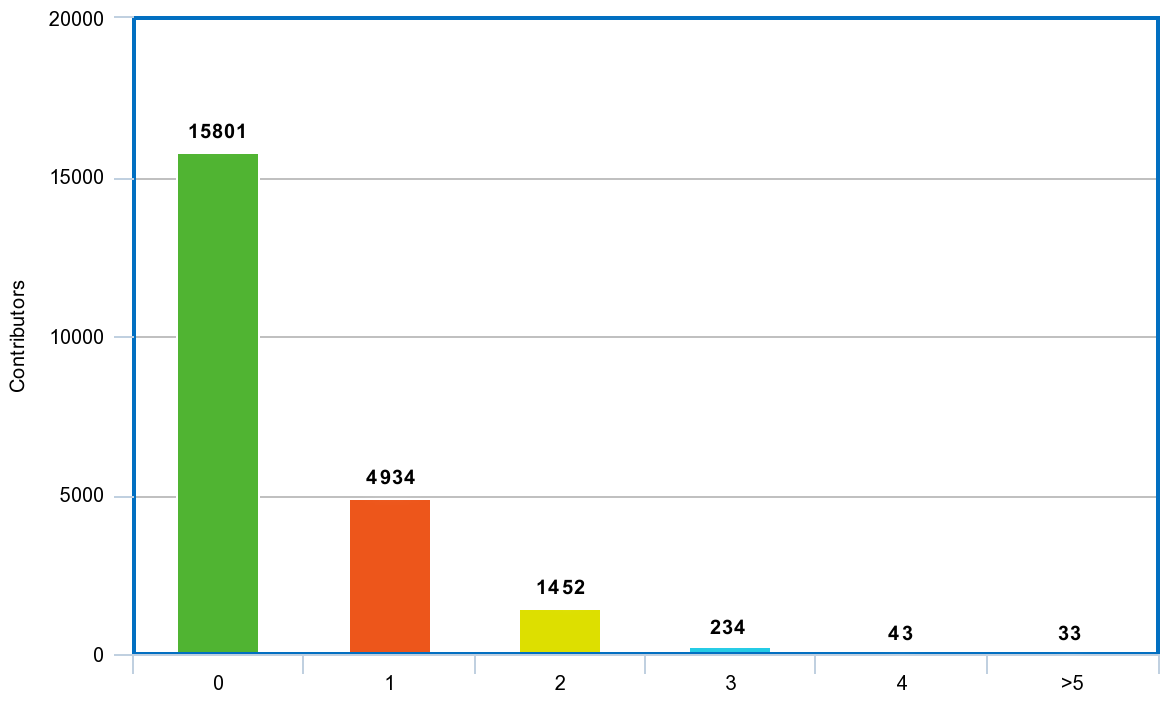
\includegraphics[scale=0.40]{./graphs/analysis/timezone-user-distribution}
    \centering
    \caption{Distribution of users according to the amount of timezone switches.}\label{fig:timezone-distribution}
\end{figure}

Figure~\ref{fig:timezone-distribution} shows the amount of contributors in relation to the amount of detected timezone switches.
On about 70\% of considered contributors only a single timezone has been detected, looking at the last year.
These 70\% do either not commit if they travel, their \acp{os} do not synchronize the timezone accordingly to their location or they simply did not travel in the last two years.

\begin{figure}[H]
    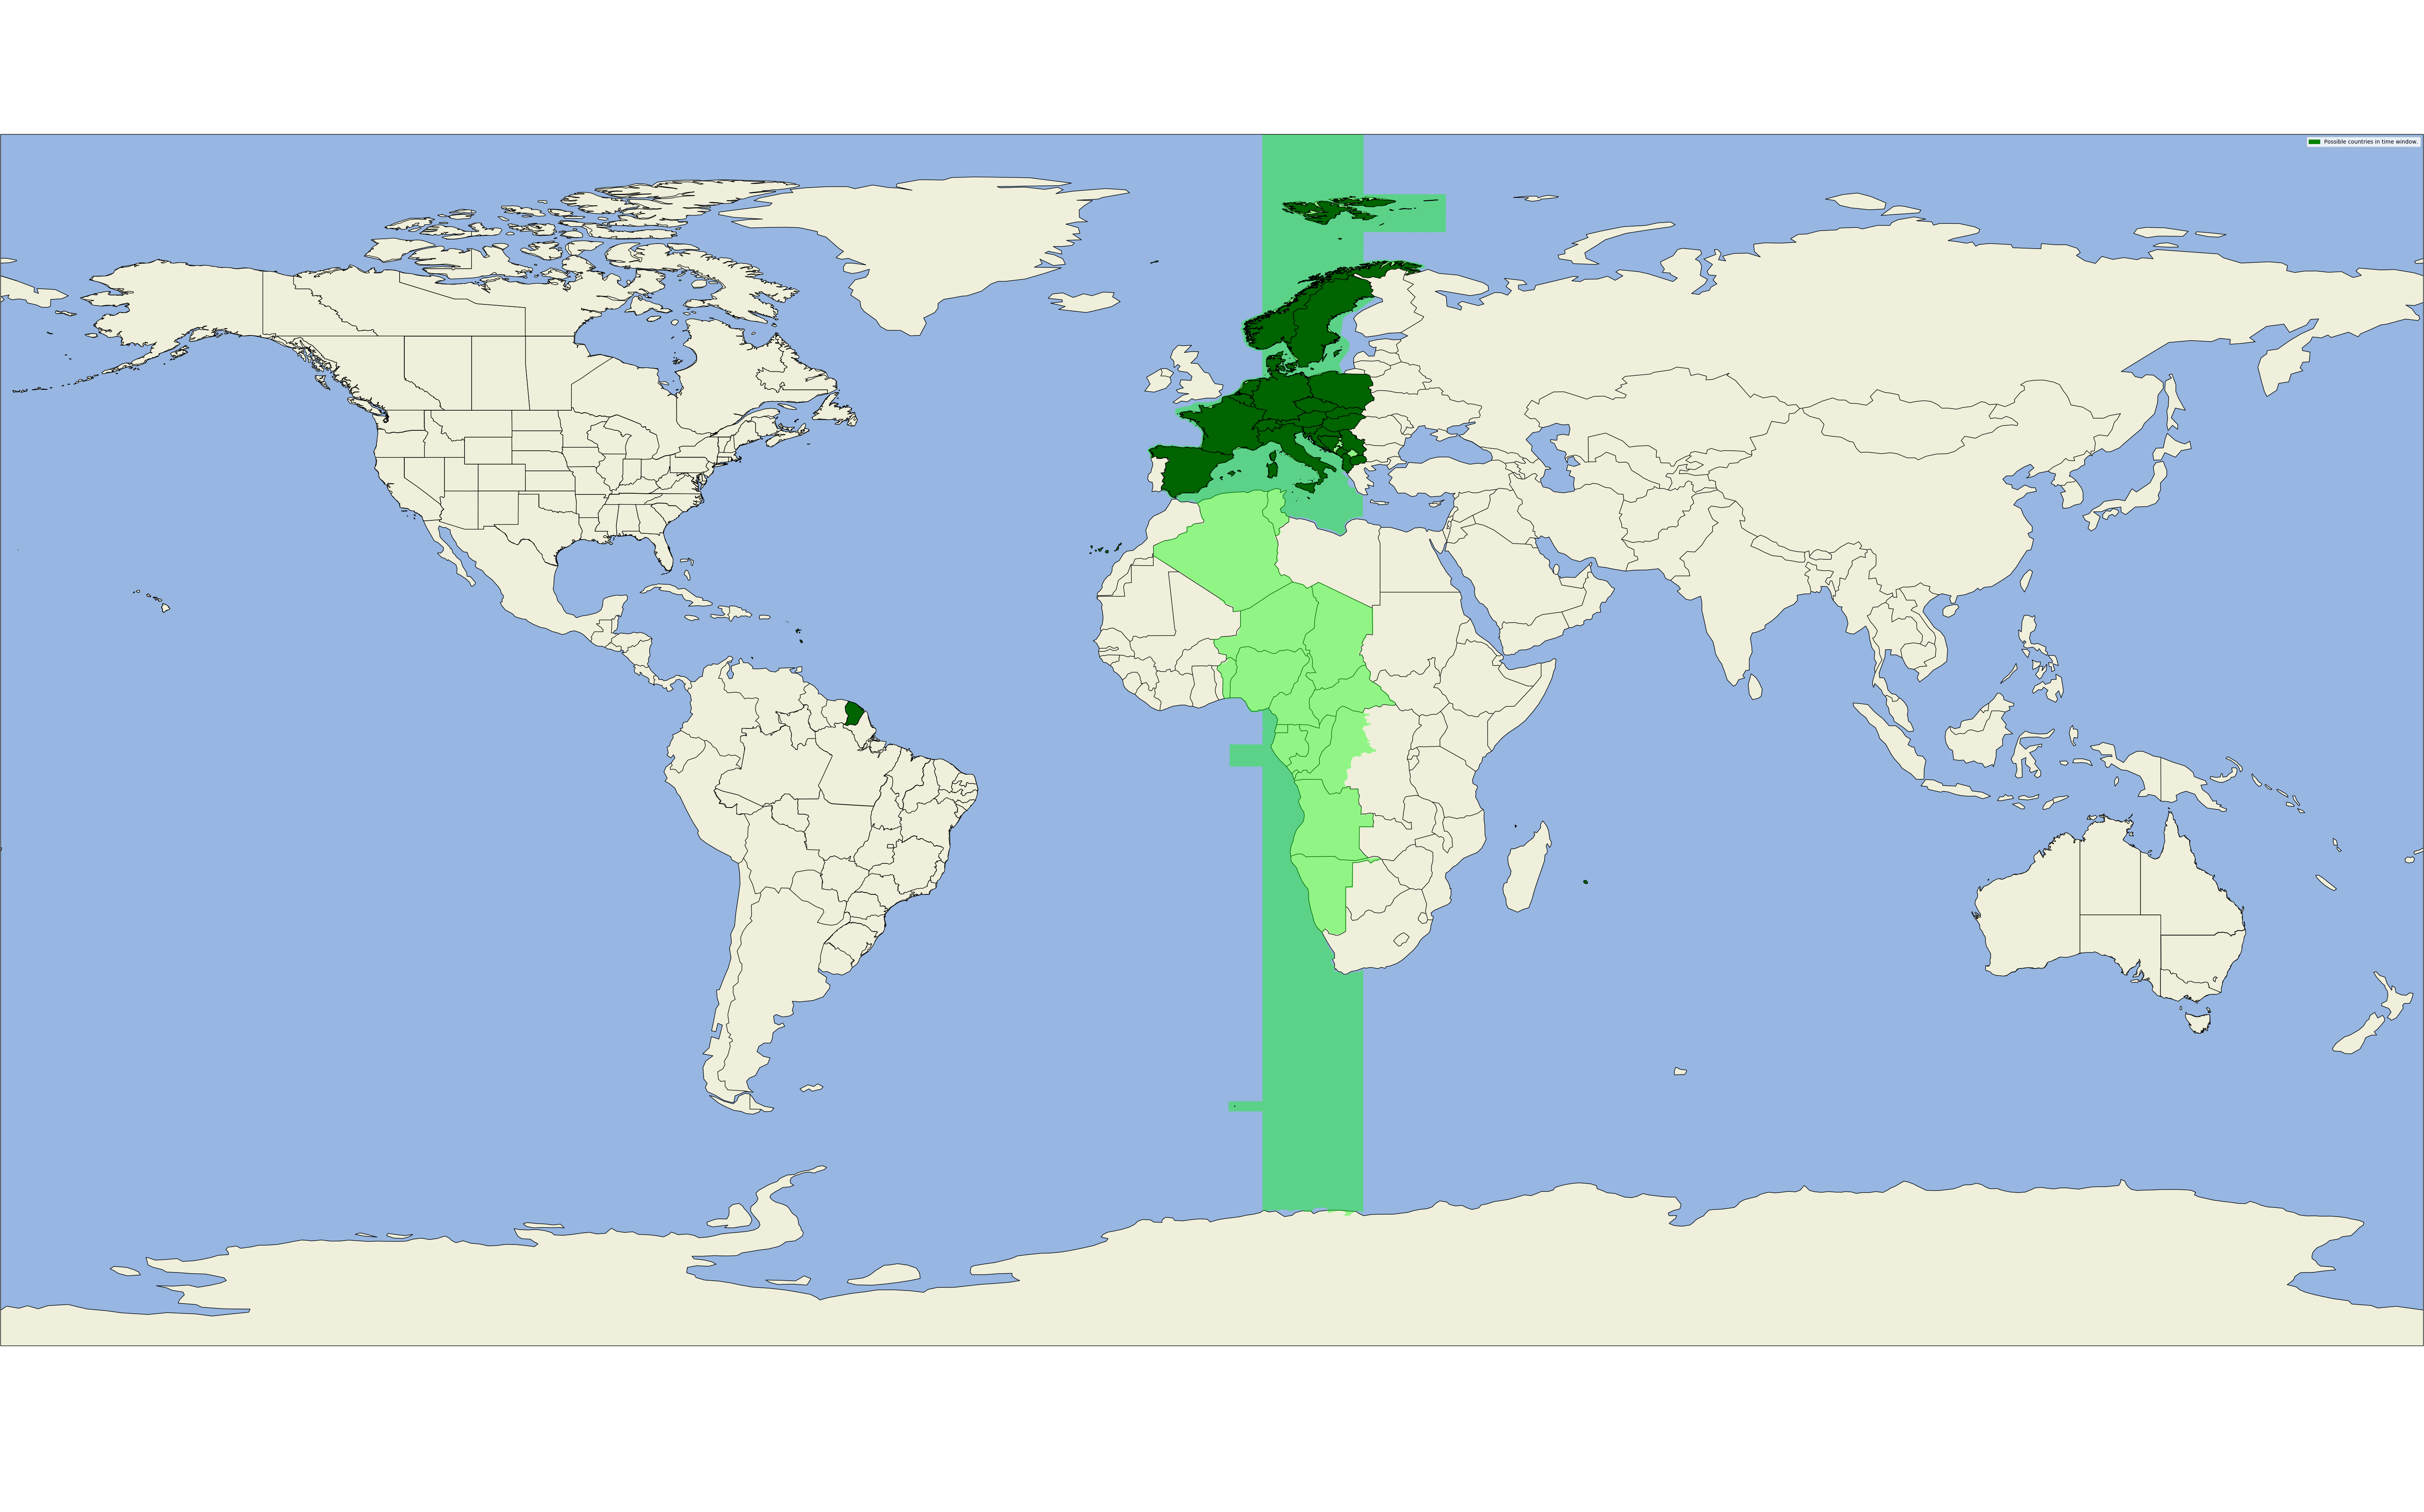
\includegraphics[scale=0.10]{./graphs/analysis/author-home-location}
    \centering
    \caption{Home location analysis of the author.}\label{fig:author-home-location}
\end{figure}

In Figure~\ref{fig:author-home-location} the visualized home location analysis of the author can be seen.
Regions marked in dark green are regions in which the contributor is likely to live.
The light green region represents the timezone of the home location.
As you can see in Figure~\ref{fig:author-home-location} the country French Guiana is also marked as a possible home location.
This problem occurs due to the several conversions between country names and codes, which were necessary as stated in Section~\ref{timezone-implementation}.
This misassignment only happens during the visualization process of the results and thereby does not affect the results of the analysis.

To evaluate the overall precision of the geolocation results, the correctness of the determined home locations are checked.
Github allows users to specify a string for their current home location, which is collected during the aggregation process.
Unfortunately there are no conventions on how this string has to look like.
Initially I tried to pass these strings to OpenStreetMap, but this resulted in too many wrongly assigned locations.
The data provided by the users was obviously too arbitrary and full of mistakes for the OpenStreetMap \ac{api} to handle.

As a result I decided to manually choose a subset of locations by looking for distinct identifiers in the location strings.
For instance, every home location of a contributor, that contained \emph{Germany} or \emph{Deutschland} in their location string, should be in the  timezone \inlinecode{Europe/Berlin}, which switches between \ac{cet} and \ac{cest}.
I created 14 such rules and was thus able to validate the home location of about 4200 contributors.
The assignment of the contributors home location was correct in about 82\% of the considered contributors.

\begin{table}[]
    \centering
    \begin{tabular}{lllll}
        Strings query        & Considered & Expected timezone    & Correct & Mean subset size \\
        & & & & \\
        San Francisco        & 772        & US/Pacific           & 639     & 12.07  \\
        NYC, NY, New York    & 485        & America/New\_York    & 366     & 23.60  \\
        India                & 148        & Asia/Colombo         & 127     & 4.01   \\
        UK, United Kingdom   & 667        & Europe/London        & 510     & 13.14  \\
        France               & 490        & Europe/Paris         & 421     & 31.59  \\
        New Zealand          & 59         & Pacific/Auckland     & 52      & 4.76   \\
        Germany, Deutschland & 976        & Europe/Berlin        & 846     & 31.48  \\
        Poland               & 180        & Europe/Warsaw        & 154     & 31.56  \\
        Italy                & 130        & Europe/Rome          & 112     & 31.39  \\
        Tokyo                & 61         & Pacific/Palau        & 48      & 8.51   \\
        Spain                & 129        & Europe/Madrid        & 116     & 32.83  \\
        Los Angeles          & 86         & America/Los\_Angeles & 76      & 12.24  \\
        Adelaide             & 2          & Australia/Adelaide   & 2       & 4.00   \\
        Mexico               & 13         & Mexico/General       & 7       & 11.62
    \end{tabular}
    \caption{Results of the home location evaluation}\label{home-location-table}
\end{table}

It needs to be noted, that the accuracy of this result is quite certainly deteriorated by location strings, which contain ambiguous information.
On manual review of the location strings, there were, for instance, strings such as \inlinecode{I love NYC}, which belongs to a developer living in Germany.
The result might also be deteriorated by contributors, which moved to another country in the last year, as we cannot detect those for sure.

Nevertheless an accuracy of 76\% clearly shows, that it is possible to narrow down the location of a contributor to a timezone and even to a subset of countries, see the last column in Table~\ref{home-location-table} for reference, by simply looking at the their git commit timestamps.


\chapter{Evaluation and Interpretation}\label{evaluation}
In the last chapter I showed the implementation of several possible attacks, which could be performed on the gathered data.
This Chapter will now attend to the evaluation of all results gained from these attacks.
I will present the extracted information from each algorithm and compare it to real world ground truth.
This information will be then be explained and audited in terms of precision and reliability.

\section{Holiday and Sick Leave Detection}

The goal of this attack is to detect miss-out by looking for anomalies in the work day patterns of a developer.

Due to possible fluctuations or changes in work routine, one requirement to this algorithm is the flexible detection of regular work patterns.
It must have the ability to adjust to a changing work pattern, but at the same time it needs to be capable of detecting anomalies in this pattern.

The input for this analysis is the intersection between all commits from the considered repositories and all commits from the considered contributors.
The commits' metadata used for this analysis are timestamps as well as additions and deletions in lines of code.

\begin{figure}[H]
    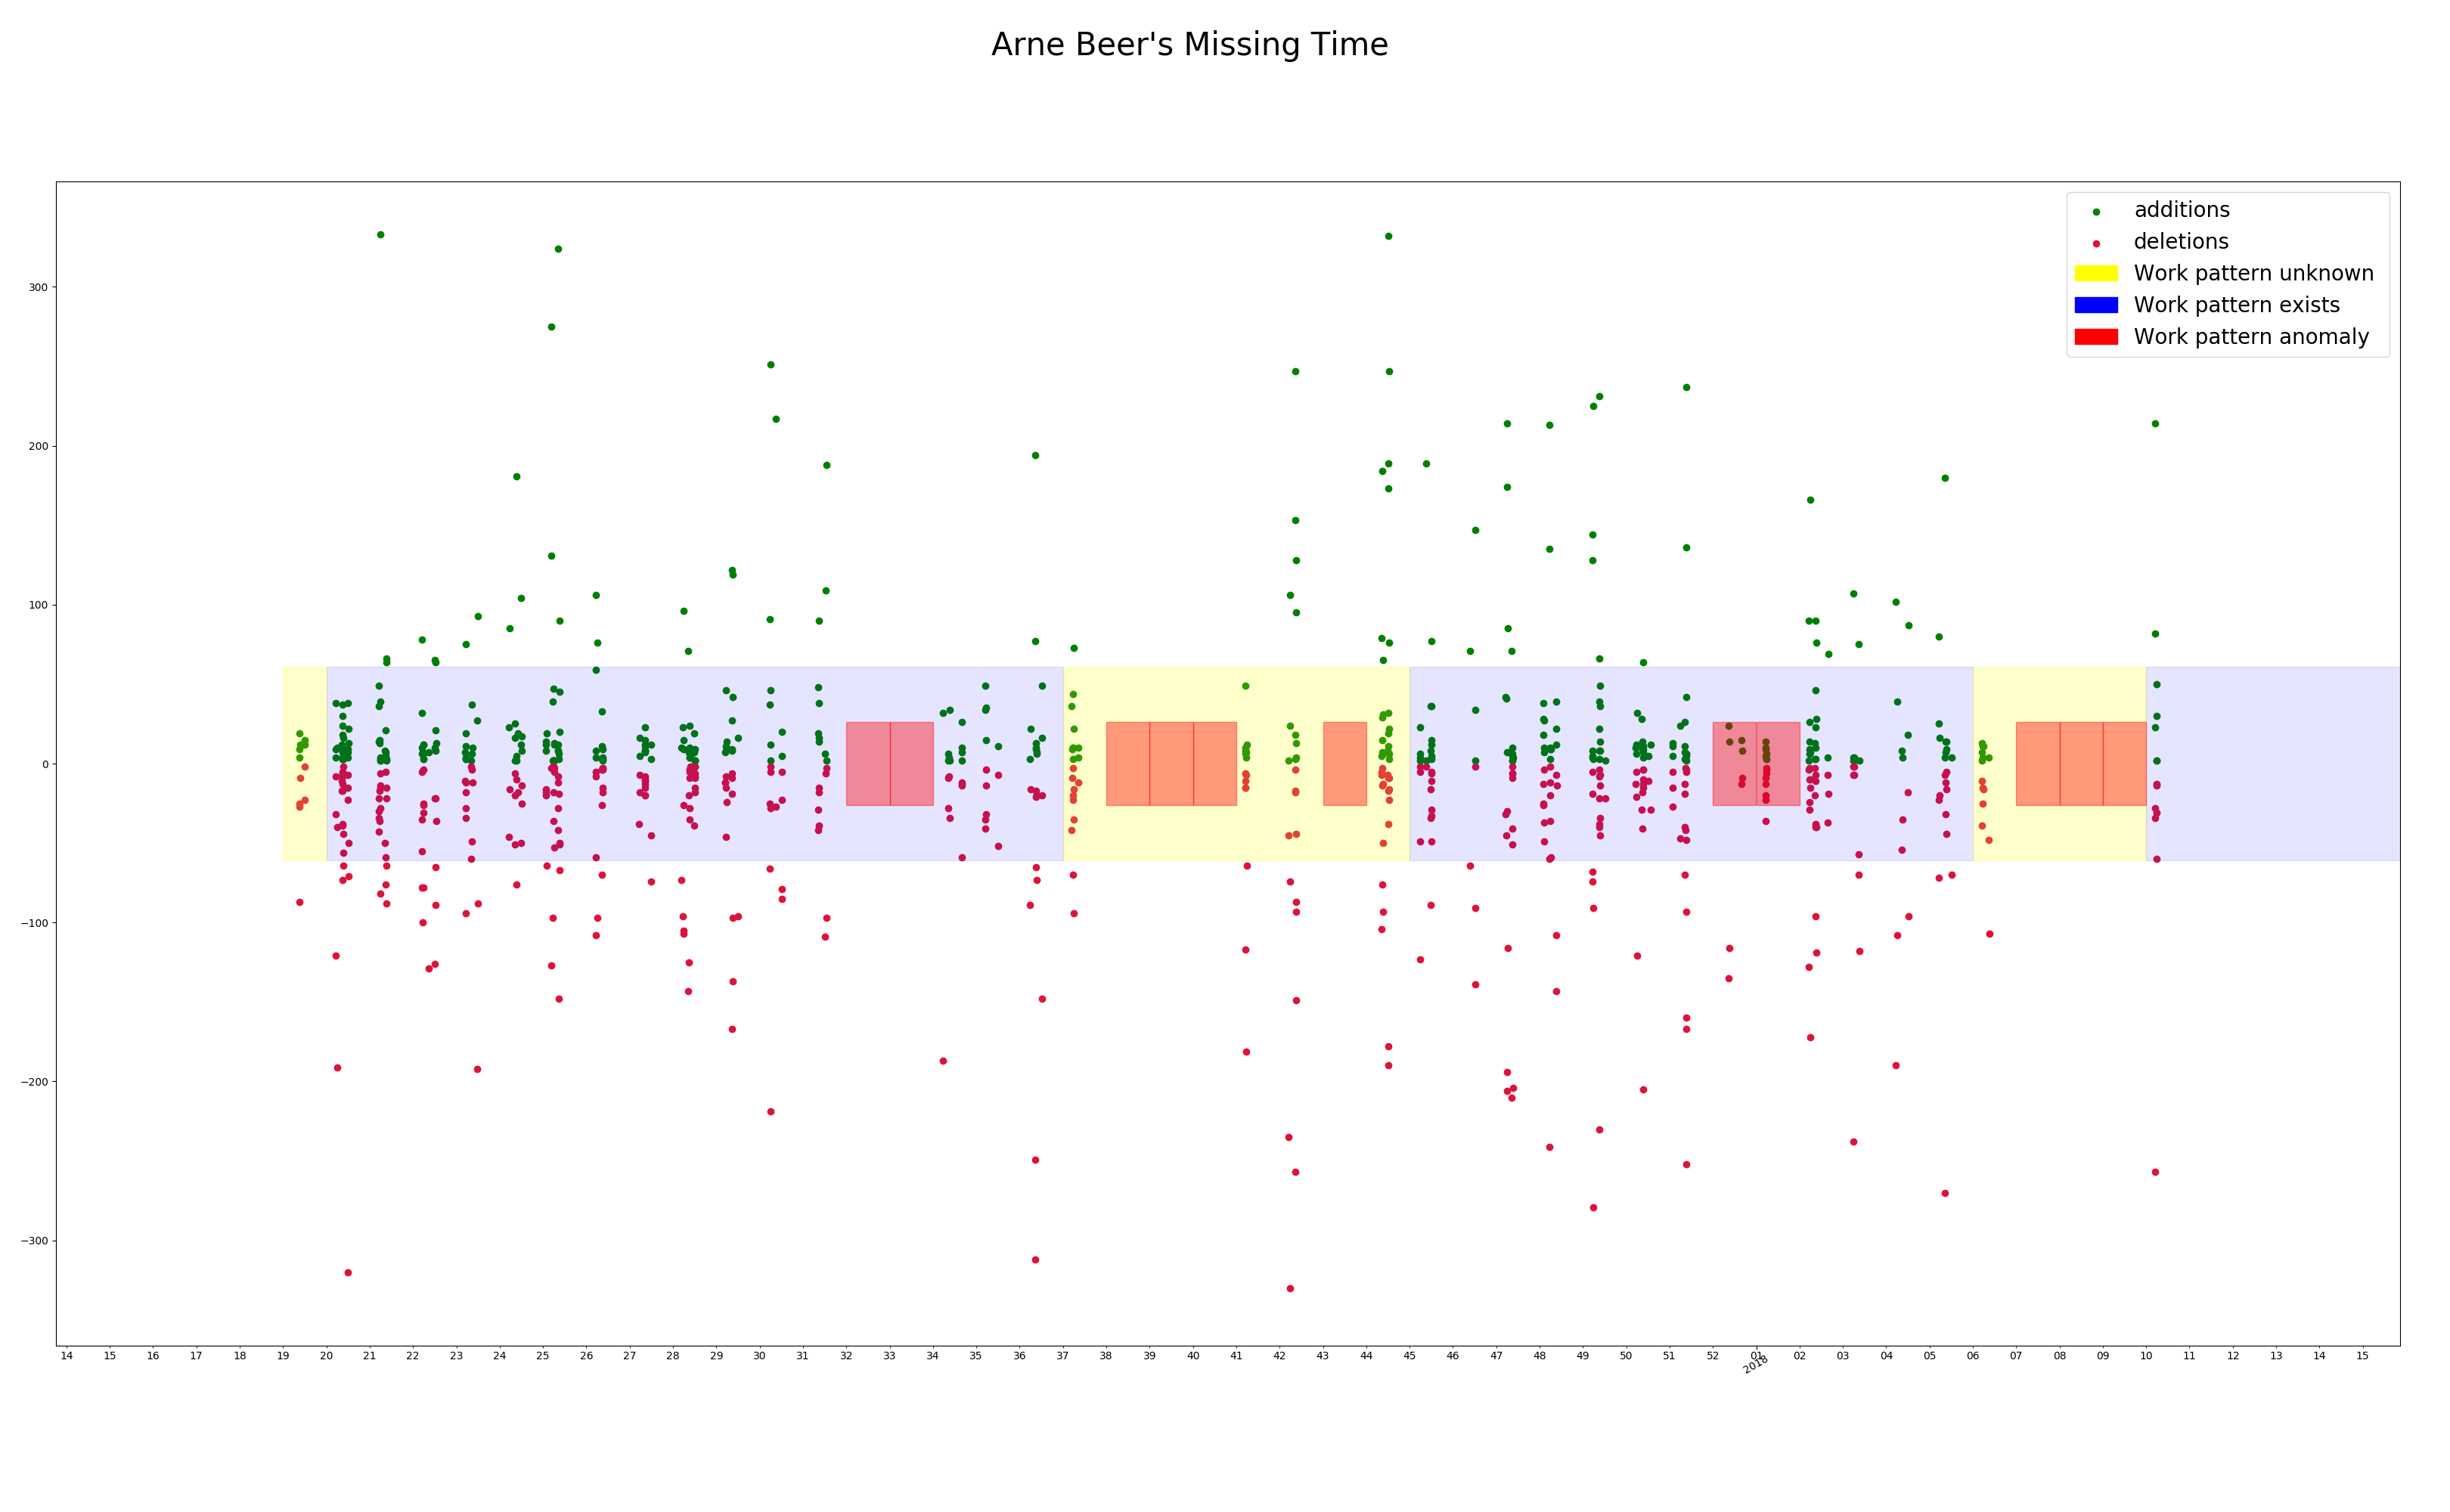
\includegraphics[scale=0.20]{./graphs/analysis/work-time-analysis}
    \centering
    \caption{The work time analysis of an employee.}\label{fig:missing-time}
\end{figure}

It is really difficult to measure productivity in lines of code or in the number of commits made by a person, as they do not necessarily display the amount of work, which has been put into this code.
As a result I decided, that a day counts as a work day as long as at least a single commit is created during the day.
Before performing the actual analysis, the data is preprocessed into an easier to handle format.
For each week of the last year a vector representing the weekdays is created.
Afterwards each day, a commit has been made on, is marked as a working day.
The preprocessed data is thereby equivalent to which days a contributor worked on, ordered by the week of the year.

\begin{minted}[linenos]{python}
def analyse(weeks):
    prototype = None
    for index, week in weeks.items():
        next_six_weeks = weeks[index:index+future_lookup]
        if not prototype:
            # Check whether there is a prototype in the next few weeks.
            prototype = find_prototype(next_six_weeks)

            # Check if this specific week is a anomaly
            check_anomaly(prototype, week)

            continue

        prototype_exists = prototype_exists_in_next_weeks(next_six_weeks)
        if not prototype_exists:
            # We couldn't find the prototype in the next few rows
            # Try to find a new prototype
            prototype = find_prototype(next_six_weeks)

        check_anomaly(prototype, week)


def check_anomaly(prototype, week):
    if week.working_days == 0:
        save_anomaly(week)

    if prototype is not None:
        different_days = week.working_days - prototype.working_days
        // A single day variance is acceptable
        if different_days >= 1:
            save_anomaly(week)

\end{minted}
\begingroup
\captionof{listing}{Miss-out analysis algorithm.}\label{lst:miss-out-algorithm}
\endgroup

The analysis of the data is a chronological scan of all work weeks for a specific user.
The algorithm inspects every week work pattern of a given interval, which has been set to a year for this analysis.
At the beginning, the algorithm tries to find a new \emph{prototype}.
A prototype is a representative week work pattern, which resembles the average work day pattern of the next weeks.
This is performed in the function \inlinecode{find\_prototype} in Listing~\ref{lst:miss-out-algorithm}.


\begin{minted}[linenos]{python}
def find_prototype(self, weeks, threshold):
    """Look at the first few weeks to find a new prototype."""
    # Create an entry for each pattern and count the occurrences of this entry
    occurrence_counter = {}
    for _, week in weeks.iterrows():
        pattern = week.pattern
        if pattern not in occurrence_counter:
            occurrence_counter[pattern] = {
                'prototype': week,
                'count': 1,
            }
        else:
            occurrence_counter[pattern]['count'] += 1

    # Get the prototype for the pattern with the most occurrences
    #
    # If there is no week which solely has the most occurences, return None.
    # In this case we can't predict a proper prototype.
    max_count = 0
    invalid = False
    prototype = None
    for _, item in occurrence_counter.items():
        if item['count'] > threshold and item['count'] > max_count:
            prototype = item['prototype']
            max_count = item['count']
            invalid = False
        elif item['count'] == max_count:
            invalid = True

    if invalid:
        return None

    return prototype
\end{minted}
\begingroup
\captionof{listing}{Miss-out analysis algorithm.}\label{lst:prototype-detection}
\endgroup

This function, which can be seen in Listing~\ref{lst:prototype-detection}, performs a simple iteration over a fix amount of future weeks, to find a work day pattern occurring more often than a given threshold.
If a prototype is found, we are capable of identifying anomalies that deviate from this pattern.

For each following week it is then firstly checked if this week is a anomaly in regards to the current prototype.
Anomalies are simply detected by comparing the amount of working days of the prototype and the considered week.
The difference in the working patterns is not suitable for this analysis, as it produces too many false positives for employees with flexible work time.

Secondly it is checked if a week identical to the prototype exists in the near future.
If there is no such week, the current prototype is reset and a new prototype needs to be found again.

In case no prototype can be found, anomalies cannot be easily identified, as there exists no pattern to check against.
Only obvious anomalies, namely weeks without a single work day, will then be marked as such.


\section{Sleep Rhythm and Working hours}

The next attack aims to extract information about the working hour behaviour of a target.
This should be achieved by displaying the pattern of the target in form of a weighted scatter plot and by comparing those patterns between several targets.
Additionally the detection of anomalies such as automated programs, which contribute to a project on a regular basis, will be conducted.

A clustering will be performed to find anomalies, common patterns and to evaluate the results of this analysis.
As we are only interested in contributors with a representative amount of commits, all contributors with less than one hundred commits in the last year have been excluded.
This reduced the amount of considered contributors from 175.000 to about 10.300.


\subsection{Implementation}\label{punchcard-implementation}

The data used for this analysis are the commit timestamps of the target, as well as the Github employee information for verification.
These commit timestamps are then converted into a different format, which represents the occurrences of commit per hour per weekday over the last year.
The result is a simple vector with length 168, which corresponds seven days with 24 hours each.
I will refer to this representation hereafter as a \emph{punchcard}.

\begin{minted}[linenos]{python}
def preprocess(commits):
    punchcard = [0] * 168
    for commit in commits:
        hour = commit.commit_time.hour # returns 0-23
        weekday = = commit.commit_time.weekday() # returns 0-6

        index = weekday*24 + hour
        punchcard[index] += 1

\end{minted}
\begingroup
\captionof{listing}{Data preprocessing}\label{lst:puchcard-preprocessing}
\endgroup

The data transformation is simply achieved by incrementing the field of the respective weekday and hour by one for each commit, as can be seen in~\ref{lst:puchcard-preprocessing}.
The resulting punchcard vector is then stored in the database for faster and easier analysis in the next steps.

\begin{figure}[H]
    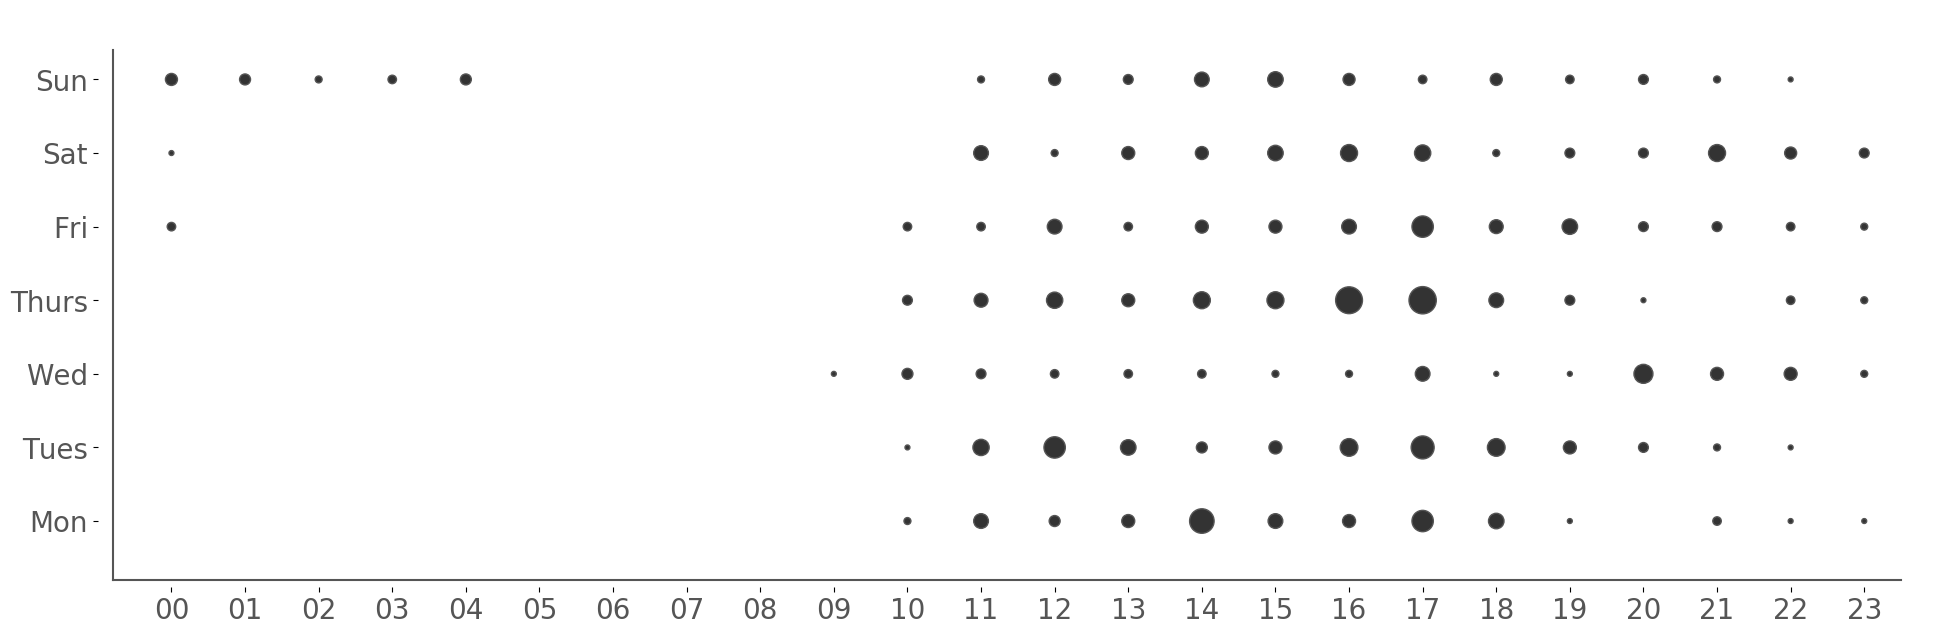
\includegraphics[scale=0.32]{./graphs/analysis/ordered-punchcard}
    \centering
    \caption{Punchcard of the author.}\label{fig:working-hour-rhythm-author}
\end{figure}


\subsection{Punchcard Clustering}

To find common work patterns, several cluster algorithms have been used on the aggregated data.
The Python \emph{scikit} framework has been used for this purpose, as it features nine different clustering methods and provides good documentation and abstraction from the underlying clustering logic~\footnote{`Clustering' scikit-learn.org, http://scikit-learn.org/stable/modules/clustering.html (accessed, 24.04.2018)}.

For the task of finding similar punchcard patterns in the data, a clustering algorithm is required, which can operate on a high-dimensional dataset with an unknown amount of clusters
Scikit provides three different clustering algorithms, which can handle an unknown amount of clusters.

\subsubsection{Mean Shift}\label{mean-shift}
Mean shift is a clustering methods, which performs an operation similar to a gradient descent, by which all adjacent data points are shifted towards their center~\cite{article:mean-shift}.
The goal of this algorithm is to find a representative centroid for each cluster and assign each data point to a cluster.
Unfortunately this methodology proves to be too aggressive for the current data.

\begin{figure}[H]
    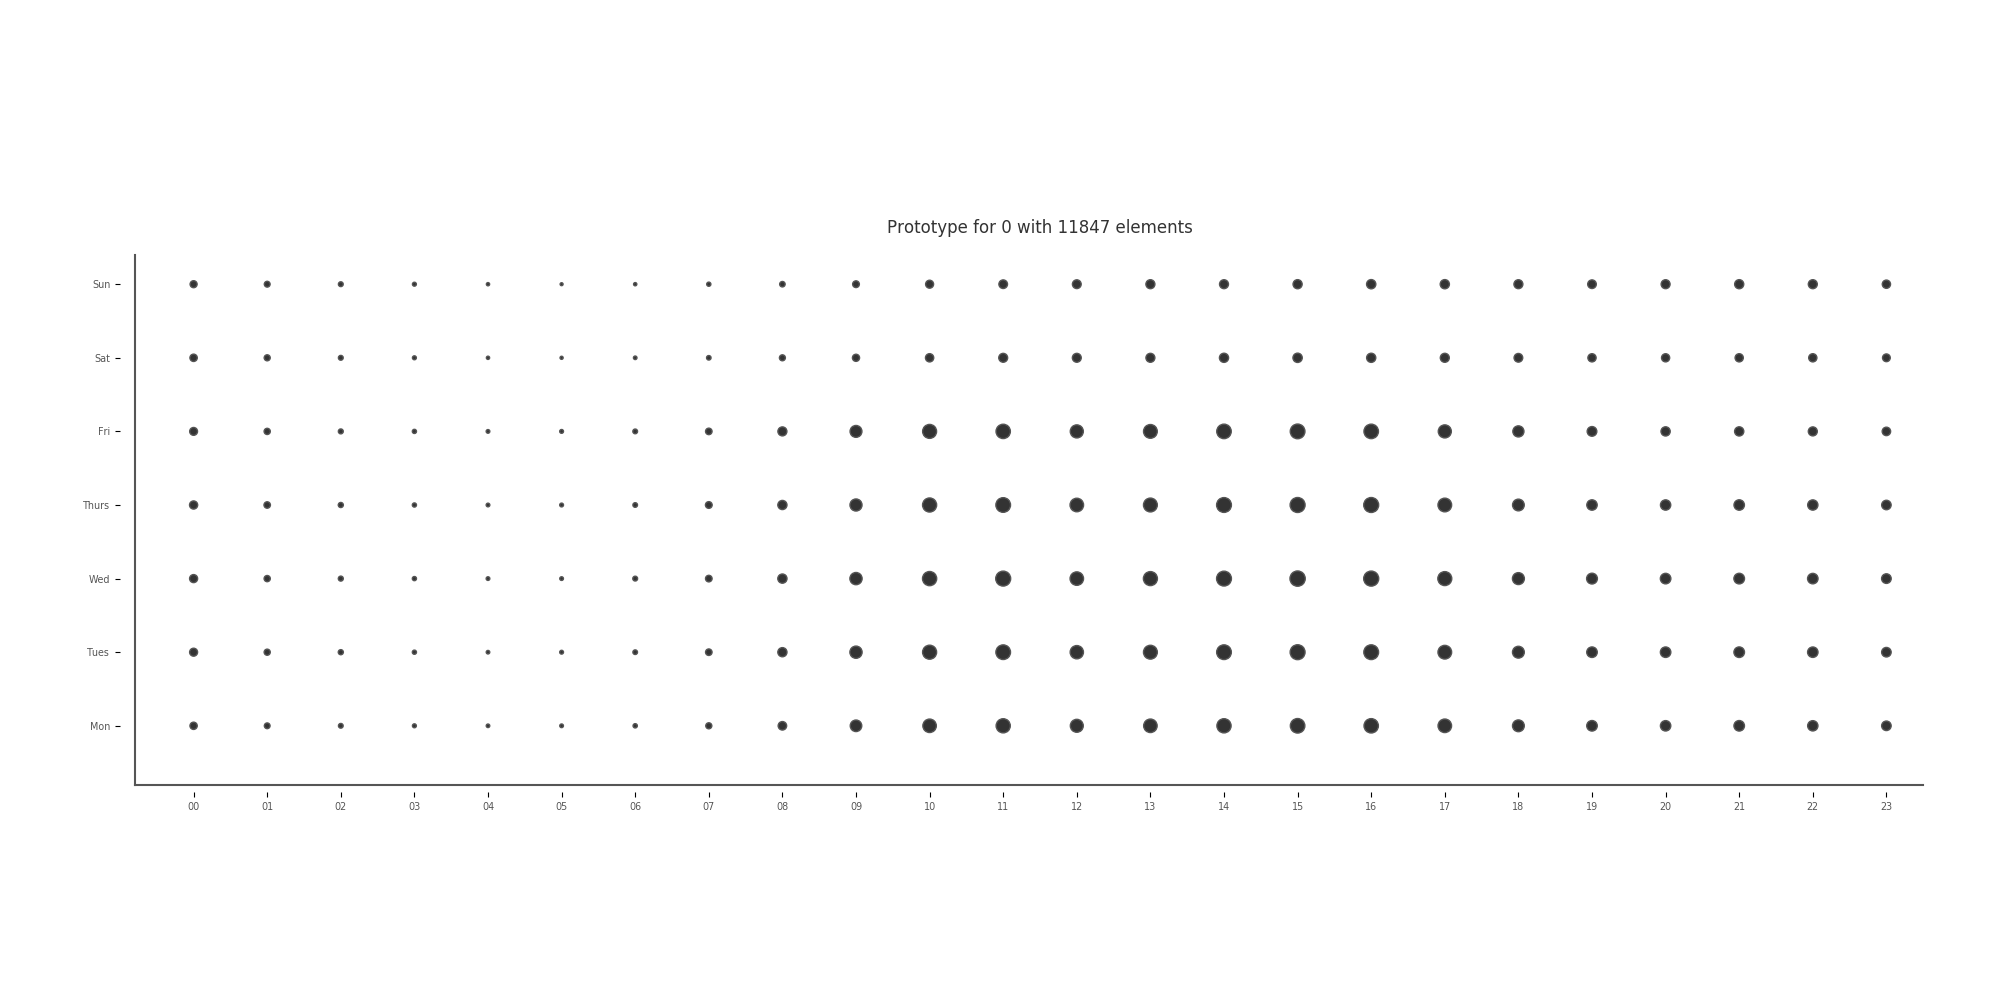
\includegraphics[scale=0.32]{./graphs/analysis-mean-shift/supercluster}
    \centering
    \caption{Super cluster centroid found by mean-shift clustering.}\label{fig:mean-shift-super-cluster}
\end{figure}

Despite trying a wide range of values for the bandwidth, which is the measure of distance used for detecting adjacent points, this algorithm always created a super cluster, which containes more than 89\% of all data points.
Such a super cluster can be seen in Figure~\ref{fig:mean-shift-super-cluster}.
The other 11\% were invariably small clusters representing extreme outlier or strange patterns, which do not resemble any of the expected patterns for normal work shift or leisure time developers.
An example for such an extreme outlier can be seen in Figure~\ref{fig:mean-shift-outlier}.

My assumption is, that the density of data points is too high and that they are too equally distributed around the centroid of the super cluster, for the major part of the provided data.
Thereby all those data points are slowly shifted to this single centroid.
As it is difficult to debug 168-dimensional space, I decided that a profound analysis would be too time consuming and to try the next solution.

\begin{figure}[H]
    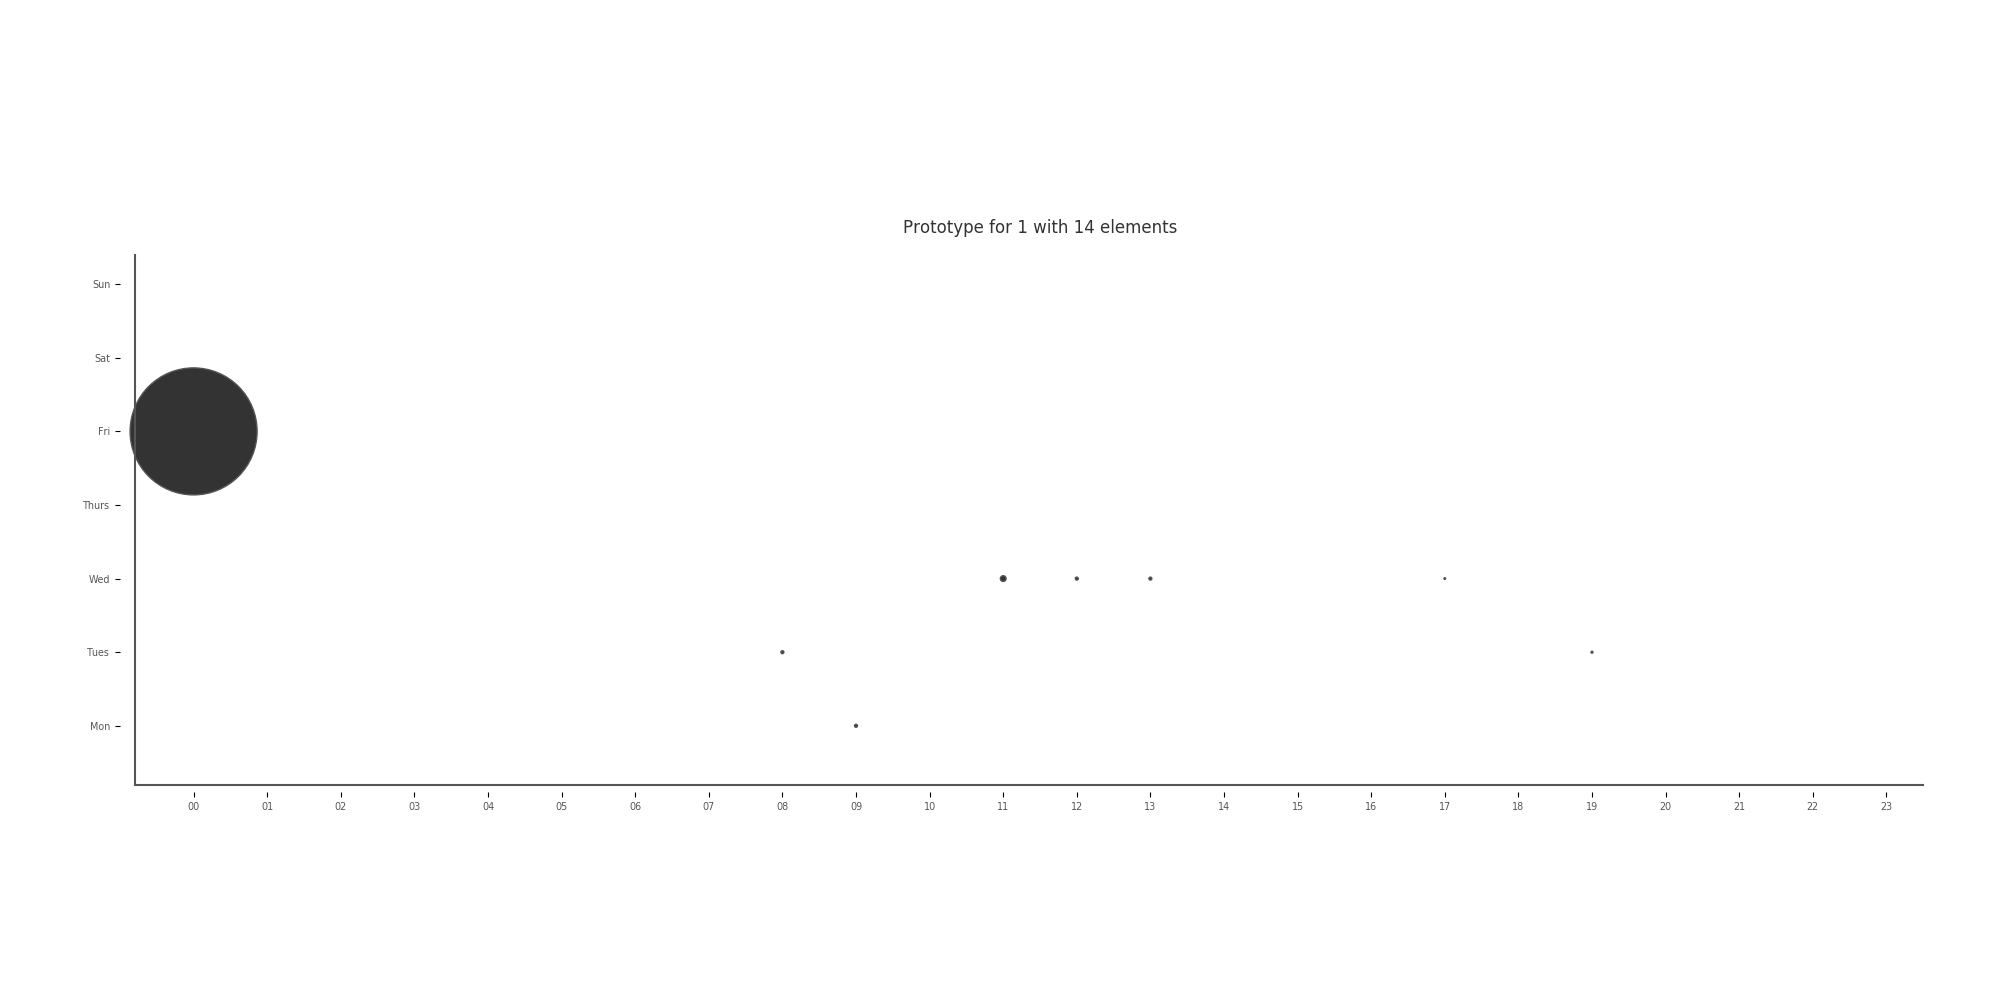
\includegraphics[scale=0.32]{./graphs/analysis-mean-shift/outlier}
    \centering
    \caption{Extreme outlier centroid found by mean-shift clustering.}\label{fig:mean-shift-outlier}
\end{figure}

\subsubsection{DBSCAN}
The \ac{dbscan} clustering algorithm operates by creating clusters of transitively connectable data points within a specific maximal acceptable distance between adjacent points.~\ref{inproceedings:dbscan}.
It is highly scalable and performant, even for large data sets, which made it my first choice.
Unfortunately it produces very similar results to the mean shift clustering algorithm~\ref{mean-shift}, since it finds a super cluster very similar to Figure~\ref{fig:mean-shift-super-cluster}.

I assume that this algorithm suffers from similar problems as the mean shift approach, which are high density and equal distribution of data points without clear borders.
Thereby the algorithm manages to reach the most part of all data points transitively from a single starting point.
When supplied with smaller values for the maximal acceptable distance between data points, it creates a huge amount of mini clusters, just as expected.

This algorithm also manages to find extreme outlier clusters, but it is not suitable for the purpose of this thesis, due to the extremely low granularity on the data inside the super cluster.


\subsubsection{Affinity Propagation}
The Affinity Propagation algorithm considers similarities between all data points to find clusters~\cite{article:affinity-propagation}.
This clustering algorithm features a promising approach, as it utilizes a method similar to message passing, to find an \emph{exemplar}, which resembles the representative of a cluster, and its surrounding cluster member.

Affinity Propagation was the only available clustering method that was detailed enough to find interesting patterns without creating a super cluster.
About 200 different patterns have been discovered using this methodology.
However it has to be noted, that this clustering method is sometimes a little too detailed, since it split very similar patterns into two or more different clusters.

Additionally, the memory requirements for this algorithm scale quadratically for non-sparse sets with the number of the data points~\cite[p.~ii]{article:affinity-propagation}.
About 12 \ac{gb} memory have already been used with a sample of roughly 10.000 data points.
This algorithm becomes thereby impractical for analyses on the whole dataset, but it works for smaller analyses and is thereby suitable for the validation of this thesis.


\section{Geolocation}

First of all, it needs to be clarified, that parts of this attack only works under specific circumstances.
Git commit timestamps are created by taking the current local time of the underlying \ac{os}.
If one wants to show the travel path of a target, the target's \ac{os} needs to automatically adjust the \ac{utc} offset accordingly to the current geolocation of the device.

This feature is available for newer versions of popular \acp{os}, such as \emph{Windows}~\footnote{Ivan Jenic, `Your Time Zone Can Now Switch Automatically in Windows 10', windowsreport.com, https://windowsreport.com/time-zone-automatic-switch-windows-10 (accessed, 24.04.2018)}
and \emph{Mac Os}, but they are not enabled by default.
It is also available for Linux, for instance with the \emph{tzupdate} package~\footnote{`Set the system timezone based on IP geolocation', github.com, https://github.com/cdown/tzupdate (accessed, 24.04.2018)}, but it needs to be manually installed and activated.

\begin{figure}[H]
    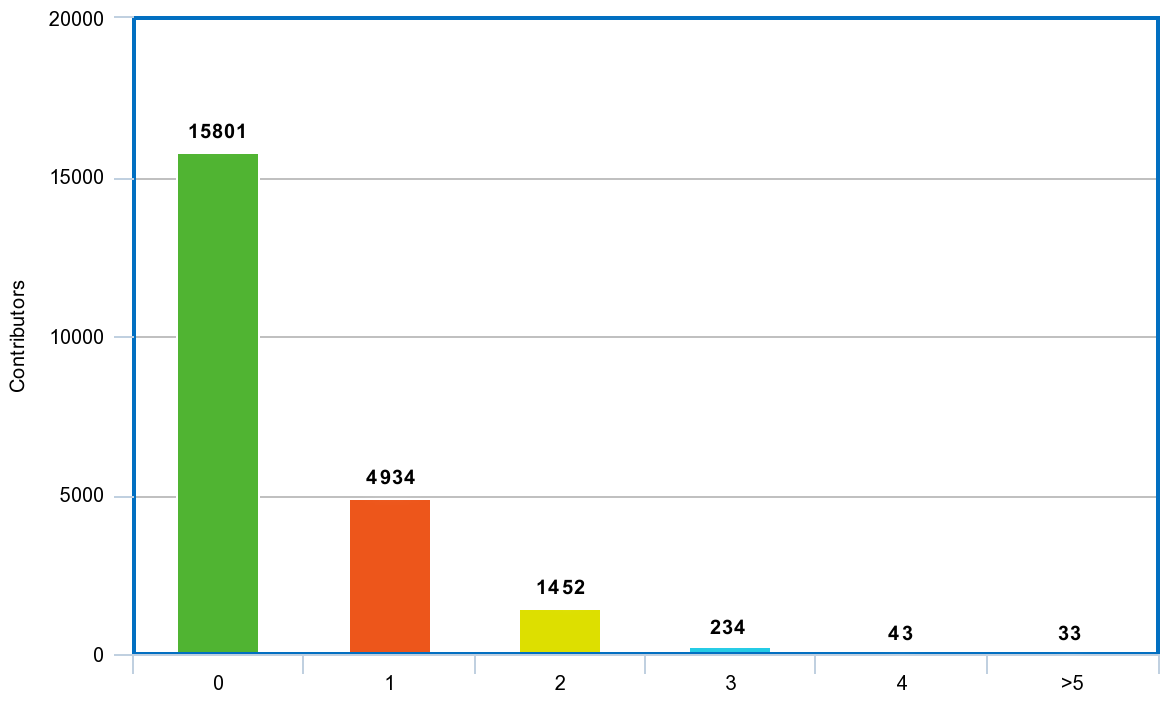
\includegraphics[scale=0.40]{./graphs/analysis/timezone-user-distribution}
    \centering
    \caption{Distribution of users according to the amount of timezone switches.}\label{fig:timezone-distribution}
\end{figure}

Figure~\ref{fig:timezone-distribution} shows the amount of contributors in relation to the amount of detected timezone switches.
On about 70\% of considered contributors only a single timezone has been detected, looking at the last year.
These 70\% do either not commit if they travel, their \acp{os} do not synchronize the timezone accordingly to their location or they simply did not travel in the last two years.

\begin{figure}[H]
    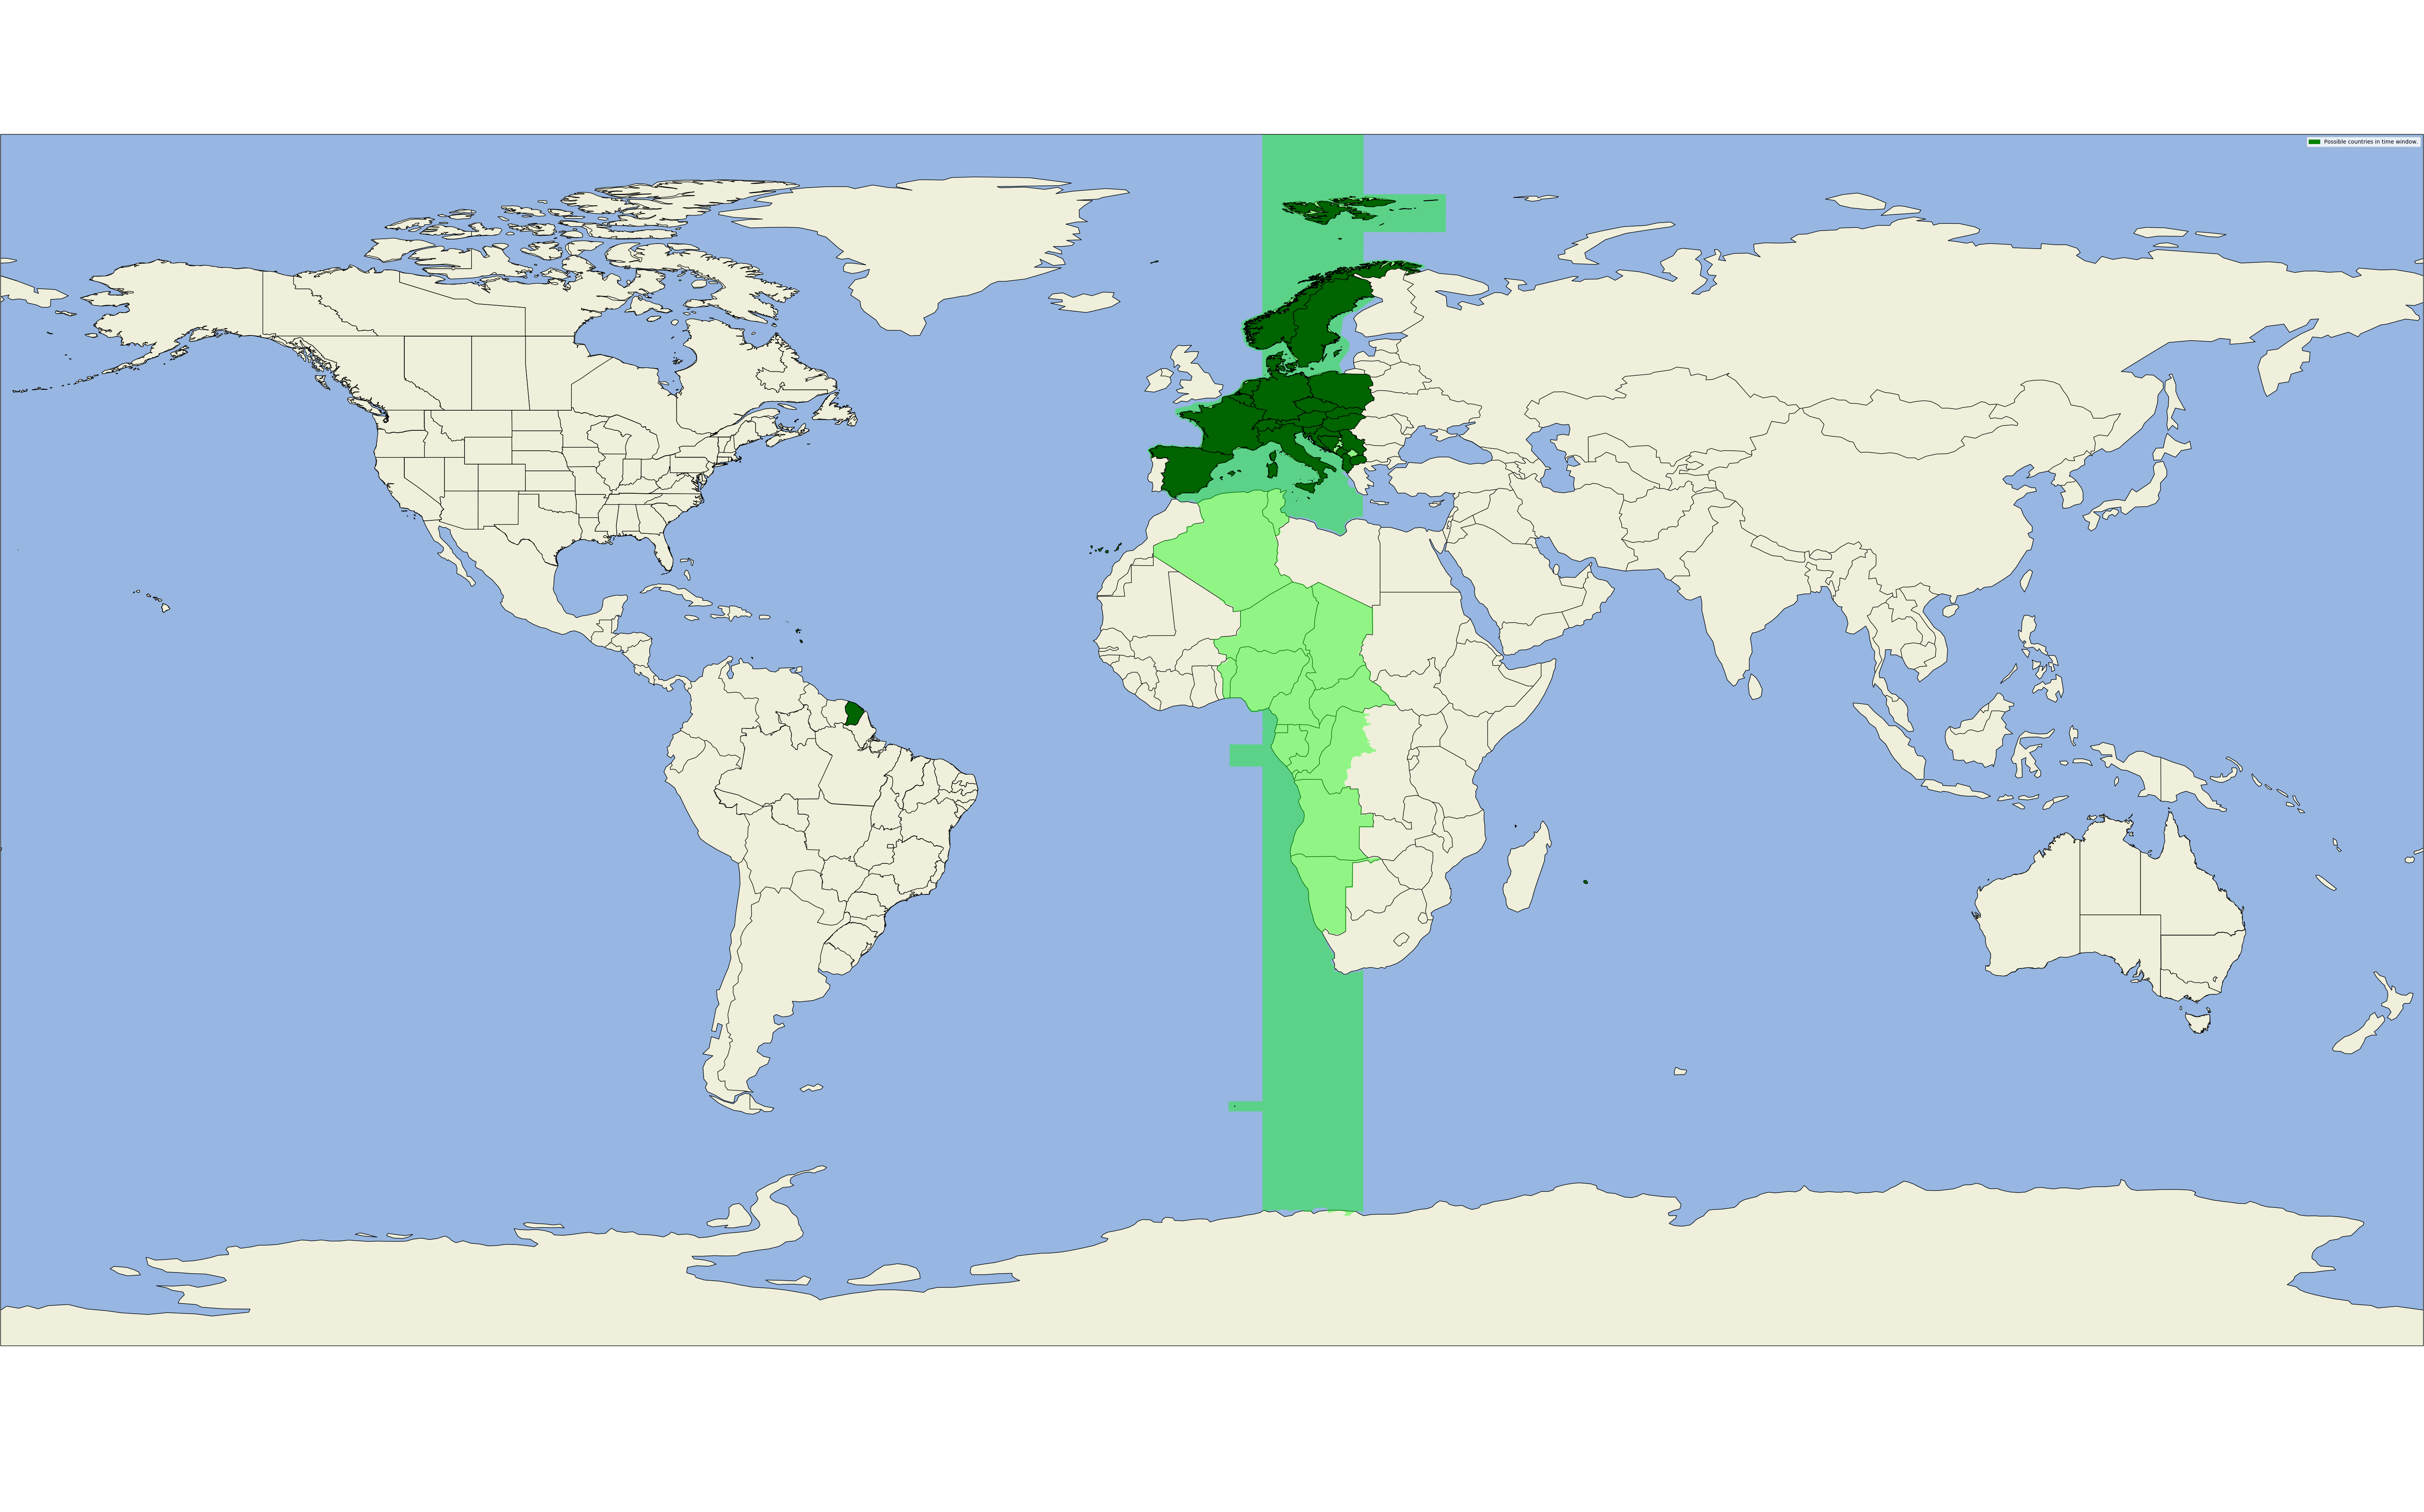
\includegraphics[scale=0.10]{./graphs/analysis/author-home-location}
    \centering
    \caption{Home location analysis of the author.}\label{fig:author-home-location}
\end{figure}

In Figure~\ref{fig:author-home-location} the visualized home location analysis of the author can be seen.
Regions marked in dark green are regions in which the contributor is likely to live.
The light green region represents the timezone of the home location.
As you can see in Figure~\ref{fig:author-home-location} the country French Guiana is also marked as a possible home location.
This problem occurs due to the several conversions between country names and codes, which were necessary as stated in Section~\ref{timezone-implementation}.
This misassignment only happens during the visualization process of the results and thereby does not affect the results of the analysis.

To evaluate the overall precision of the geolocation results, the correctness of the determined home locations are checked.
Github allows users to specify a string for their current home location, which is collected during the aggregation process.
Unfortunately there are no conventions on how this string has to look like.
Initially I tried to pass these strings to OpenStreetMap, but this resulted in too many wrongly assigned locations.
The data provided by the users was obviously too arbitrary and full of mistakes for the OpenStreetMap \ac{api} to handle.

As a result I decided to manually choose a subset of locations by looking for distinct identifiers in the location strings.
For instance, every home location of a contributor, that contained \emph{Germany} or \emph{Deutschland} in their location string, should be in the  timezone \inlinecode{Europe/Berlin}, which switches between \ac{cet} and \ac{cest}.
I created 14 such rules and was thus able to validate the home location of about 4200 contributors.
The assignment of the contributors home location was correct in about 82\% of the considered contributors.

\begin{table}[]
    \centering
    \begin{tabular}{lllll}
        Strings query        & Considered & Expected timezone    & Correct & Mean subset size \\
        & & & & \\
        San Francisco        & 772        & US/Pacific           & 639     & 12.07  \\
        NYC, NY, New York    & 485        & America/New\_York    & 366     & 23.60  \\
        India                & 148        & Asia/Colombo         & 127     & 4.01   \\
        UK, United Kingdom   & 667        & Europe/London        & 510     & 13.14  \\
        France               & 490        & Europe/Paris         & 421     & 31.59  \\
        New Zealand          & 59         & Pacific/Auckland     & 52      & 4.76   \\
        Germany, Deutschland & 976        & Europe/Berlin        & 846     & 31.48  \\
        Poland               & 180        & Europe/Warsaw        & 154     & 31.56  \\
        Italy                & 130        & Europe/Rome          & 112     & 31.39  \\
        Tokyo                & 61         & Pacific/Palau        & 48      & 8.51   \\
        Spain                & 129        & Europe/Madrid        & 116     & 32.83  \\
        Los Angeles          & 86         & America/Los\_Angeles & 76      & 12.24  \\
        Adelaide             & 2          & Australia/Adelaide   & 2       & 4.00   \\
        Mexico               & 13         & Mexico/General       & 7       & 11.62
    \end{tabular}
    \caption{Results of the home location evaluation}\label{home-location-table}
\end{table}

It needs to be noted, that the accuracy of this result is quite certainly deteriorated by location strings, which contain ambiguous information.
On manual review of the location strings, there were, for instance, strings such as \inlinecode{I love NYC}, which belongs to a developer living in Germany.
The result might also be deteriorated by contributors, which moved to another country in the last year, as we cannot detect those for sure.

Nevertheless an accuracy of 76\% clearly shows, that it is possible to narrow down the location of a contributor to a timezone and even to a subset of countries, see the last column in Table~\ref{home-location-table} for reference, by simply looking at the their git commit timestamps.



\begingroup
    \footnotesize
    \listoffigures
    \let\clearpage\relax
    \listoflistings{}
    \listoftables
\endgroup

\renewcommand*{\bibfont}{\footnotesize}
\printbibliography{}


\chapter*{Eidesstattliche Erklärung}
\onehalfspace{}
„Hiermit versichere ich an Eides statt, dass ich die vorliegende Arbeit im
Studiengang Informatik selbstständig verfasst und keine anderen als die
angegebenen Hilfsmittel – insbesondere keine im Quellenverzeichnis nicht
benannten Internet-Quellen – benutzt habe. Alle Stellen, die wörtlich oder
sinngemäß aus Veröffentlichungen entnommen wurden, sind als solche kenntlich
gemacht. Ich versichere weiterhin, dass ich die Arbeit vorher nicht in einem
anderen Prüfungsverfahren eingereicht habe und die eingereichte schriftliche
Fassung der auf dem elektronischen Speichermedium entspricht.“
\singlespace{}

\vspace{1cm}

\begin{tabular}{ll}
    \centering
    \makebox[5cm]{\hrulefill} & \makebox[5cm]{\hrulefill}\\
    Ort, Datum & Unterschrift \\
\end{tabular}


\end{document}
